\documentclass[12pt,titlepage]{article}

\usepackage{etex}
\usepackage[english]{babel}
\usepackage[utf8]{inputenc}
\usepackage[T1]{fontenc}
\usepackage{color}
\usepackage[a4paper,lmargin={4cm},rmargin={3cm},tmargin={3cm},bmargin={3.5cm}]{geometry}
\usepackage[onehalfspacing]{setspace}
\usepackage{amssymb}
\usepackage{amsthm}
\usepackage[pdftex]{graphicx}
\usepackage{lmodern}
\usepackage{amsmath}
\usepackage{amsfonts}
\usepackage{multirow}
\usepackage{rotating}
\usepackage{mathrsfs}
\usepackage{graphicx}
\usepackage{tikz}
\usepackage{makecell}
\usepackage{vcell}
\usepackage{arydshln}
\usepackage{textcomp}
\usepackage{diagbox}
\usepackage{caption}
\usepackage{subcaption}
\usepackage{algpseudocode}
\usepackage{algorithm}
\usepackage{relsize}
\DeclareCaptionType{equ}[][]
\usepackage[style=numeric]{biblatex}
\addbibresource{literaturechurn.bib}
\usetikzlibrary{trees}
\graphicspath{{./images/}}
\DeclareMathOperator*{\argmin}{arg\,min}


\begin{document}

\thispagestyle{empty}

\begin{titlepage}\centering
    \begin{center}
        \vspace*{\fill}
        \huge \textbf{\textsf{Customer Churn Prediction using Quotation Data}}\\
        \vspace{2cm}
        \LARGE\textbf{\textsc{Master Thesis}}\\
        \vspace{1cm}
        \normalsize
        Submitted on: \today \\
        \vspace{2.5cm}
        \large \textbf{at the University of Cologne}
        \vspace{3cm}
    \end{center}
    \normalsize{
        \begin{tabular}{ll}
            Name: & {Abdurahman Maarouf} \\
            Adress: & {Schulstrasse 31} \\
            Postcode, Area: & {53332, Bornheim} \\
            Country: & {Germany} \\
            Matriculation number: & {736481} \\
            Supervisor: & {Prof. Dr. Dominik Wied} \\
        \end{tabular}\\
    }
    \vspace*{\fill}

\end{titlepage}

\thispagestyle{empty}

\tableofcontents

\newpage

\pagenumbering{arabic}

\setcounter{page}{1}

\section{Introduction} \par

Predicting churners in order to retain customers has become one of the most important issues for companies in the field of Customer-Relationship-Management. With the exponential rise of data availability in the recent two decades, companies develop tools and methods to detect potential churners before they leave. More precisely, their goal is to estimate probabilities for a churn per customer in the next period of time. To tackle this issue, more and more advanced Machine-Learning-Algorithms are used guaranteeing solid accuracy in their out-of-sample predictions. \\
Fortunately for most of the companies, churn rates from one period to another are very small. However in classification
models predicting a rare event can become challenging. In this so called "Imballanced Classes" issue certain arrangements to the underlying training data or the selected loss function need be made. Without these arrangements and with highly imballanced classes, a poor algorithm simply never predicts the outcome of the minority class. In a dataset with 1000 customers containing 5 churners for example, this loss-minimizing algorithm would have an accuracy of 99.5\%. \\
In order to avoid the high amount of false-negative classifications there are many methods ranging from upsampling the
minority class or downsampling the majority class to more advanced techniques like custom loss functions. In this work we present and compare the different methods while applying them to the underlying problem. \\
In this work we want to emphasize the importance of using quotation data for predicting customer churn. A company can
track (potential) customer behavior on their distribution channels. Nowadays, in most cases the products or services are
offered online on websites, which makes it easy to track website visitor data. In the context of dealing with customer
churn this data can be matched to the customers already having a product or contract of this company. We show that first the number of visits of a current customer in the last period and second the average of the seen price during the visits have a high importance when predicting the probability of that customer leaving in the next period. \\
Another task of this work is to evaluate and interpret the importance and relationship of not only the quotation variables but also the other explanatory variables with the predicted outcome. In terms of explainability and interpretability, there is typically a trade-off during model selection. The trade-off lies between the model complexity and the model interpretability. Gradient boosted trees (GBT) belong to the complex models which are famous for their comparatively high accuracy in almost all domains involving tabular data applications. Explaining and interpreting the resulting GBT by its model structure becomes almost infeasable. \\
However in the course of this work and in many other areas understanding how explanatory variables interact with the outcome of the model becomes desirable. Knowing what the main drivers for high churn probabilities are can increase the scope of action the company has for retention strategies. The most transparent models in terms of interpretability are linear or logistic models. There the magnitude and sign of the corresponding coefficients (after being testet for significance) illustrate the changes of the outcome for a change in the specific explanatory variable. These models lack in terms of predictive performance when being compared to the complex ones, because they do not allow for non-linearities and interactions in the explanatory variables. Extensions, like general additive models (GAMs) \cite{gam} or GAMs allowing for pairwise interactions (GA$^{2}$Ms) \cite{ga2m} incorporate non-linearities.\\
In this work we focus on comparing (1) the predictive performance and (2) interpretability of black-box and white-box models. For the black-box model we fit GBTs \cite{gbt} as they outperform other models in most applications with tabular data. Partial dependency plots \cite{pdp}, Shapley values \cite{shap} and LIME \cite{lime} are novel approaches designed to make these black-box models interpretable. Additionally we present "Explainable Boosting Machines" (EBM) developed by Microsoft researchers Lou et al. \cite{interpretml} which are based on GA$^{2}$Ms and are therefore interpretable in the form of their shape functions. EBMs aim to combine the high predictive performance of complex models on the one hand and the interpretability of general additive models on the other hand. \\

\section{Problem} \par

\subsection{Understanding the Problem} \par

For this work we use an applied problem of a big insurance company in Germany. Due to data pretection the real data is not used. We however provide a sample data set, which resembles the real data in distribution, variables and statistical relationships. We focus on the product of automobile liability insurance, which is by law a mandatory service every car owner must hold in Germany. \\
Typically car owners close a deal with an insurance company which can be terminated by the end of each year. In rare cases both sides agree on a contract with a due date during the year. If the contract does not get terminated it is automatically extended for another year. Besides the option to terminate the contract at the due date there is also an option to terminate it earlier in a few special cases. These cases mainly involve the exceptional right of termination given to a customer. Here are the two most frequent reasons for this exceptional right, in which a churn can (but not must) occur before the contract due date: \\

\noindent
\begin{center}
    \begin{tabular}{ll}
        Event A: & Contractor is involved in an Accident. \\
        Event N: & Contractor buys a new Car. \\
    \end{tabular}
\end{center}

\vspace{3mm}
\noindent
The problem of predicting churn needs to be seperated into the probability of a costumer leaving before his contract due date and churns happening at the due date. The reason is that the optimal modelling approach and explanatory variables have proven differences. One example is the premium adjustment send to the customers before their due date, which has a high contribution to the decision of the customers at the due date. Meanwhile, churns before the due date are dependent on the occurence of the events $A$ and $N$. In this work we focus on predicting churns occuring before the due date. \\

The purpose is to build a model which can be used at any time $t$ of the year to predict the probability of a costumer leaving the company in the next period of time $(t, t+s]$ and not at his due date. It can be argued that in order to provide a model with maximized utility for production one would want to keep $s$ small. For example a company would highly benifit from a model, which can predict the churn-probability of the next week. However we see that having a small $s$ decreases the accuracy of our models, creating a trade-off situation between model accuracy and the benifits of a small $s$. With a smaller period the classes of the data become more imballanced, creating a higher challange of feeding the model enough information about churners. Furthermore, a small $s$ decreases the scope of action for a company to retain potential customers leaving. \\

\subsection{Idea} \par

This work stands out in its novel approach of using quotation data for churn predictions. We are not aware of similar research in the literature utilizing that type of data. In the following we clarify what our understanding of quotation data is. \\
Through every distribution channel a company offers its product, (potential) customers leave behind a lot of useful data. These distribution channels can either be online websites or also offline agencies. In our insurance application (potential) customers must give specific information about themselves and their car they want to insure such that a price can be calculated. Everytime a price is calculated all the information corresponding to that calculation is saved as a new row on the companies' database. From now on we define a price calculation as a request. \\
Main applications of quotation data involve price and new-business optimization, demand forecasting and conversion modelling. Another application however is to use this data in order to analyze the behavior of customers which already have an active contract. The main advantage is that (potential) customers having to enter their and the cars information. This entered information can be used to match an active customer with his/her requests. \\
In a prediction model information generated from quotation activity of time period $(t-m, t]$ can be used as explanatory variables. What type of quotation variables we generate is explained in chapter \ref{chap:dataprep}. \\
\subsubsection*{Hypothesis}
The hypothesis of this work is that an active customer with high request activity is most likely looking for a new insurance contract. This would directly influence the churn probability. We test this hypothesis by: (1) Evaluating model predictions on unseen data with and without quotation data (2) Interpreting the models in terms of relationship between quotation variabes and predicted outcome. \\

\subsection{Literature Review} \par

There is a wide range of literature covering supervised classification techniques and their usage for customer churn prediction. Verbeke et al. \cite{verbekechurn} provides an overview table on the literature dealing with churn modelling in static settings using cross-sections of data. It provides an extensive benchmark of classification methods and machine learning models applied to different data sets. \\
Some works have a different approach in modelling customer churn. Van den Poel et al. \cite{vandenpoel} for example models the time to churn using survival analysis techniques. This allows flexible estimations for the conditional probability of customer $i$ churning in the next $s$ periods of time, where the probability can be calculated for different values of $s$ by the model structure itself. Given the fact that with survival analysis, conditioning on multiple time dependent variables is not possible or not well studied yet, we focus on modelling churn probabilities in the static setting. \\
The popularity of (deep) neural networks has risen enormously in the last two decades. Its promising accuracy in computer vision, natural language processing and sequential data in general are the reasons for its broad coverage in research. It has also found its way to modelling customer churn, as in \cite{martins}, \cite{tan2018}, \cite{wangperawong}, \cite{zaratiegui}, \cite{zhou} and \cite{mena}. All cited papers rely on the fact that customer data can be used as sequential data with time varying variables. Therefore model architectures like convolutional neural networks (CNN) and long short-term memory networks (LSTM) come into play. We however focus on classification techniques which do not assume dependencies in the data points, given the data that we have available. \\
The different data preparation, preprocessing and variable engineering approaches for churn modelling are also extensively studied. \cite{coussement} for example studies the data preparation approach for modelling churn probabilities in the telecommunication industry. They suggest that an appropriate selection and engineering of variables is essential to guarantee robust results and high accuracy. We apply their suggestion to some of our variables, which however differ due to the different setting. \\
Regarding preprocessing, Gattermann-Itschert et al. \cite{multiplets} underline the importance of multi-slicing. This technique essantially uses multiple time-slices $T$ in the past to train the underlying models. They find out that this technique results in higher accuracy and robustness, which also holds true for our application. \\
As already stated, class imbalance naturally occurs in most churn prediction applications due to the fact that churners are less frequent than non-churners. This problematic increases in a contract setting, where there are only a few events which allow for an earlier termination than the due date. Weiss et al. \cite{mining_rarity} provides an overview on multiple techniques to handle class-imbalance. It espacially highlights the effectiveness of sampling and cost-sensitive learning which prove to be the best techniques in our application as well. \\
Zhu et al. \cite{zhu} offers a useful guideline of sampling methods in the context of churn prediction. It compares different sampling techniques in their effectiveness and multiple evaluation metrics. Burez et al. \cite{burez} extensively underlines the importance of using appropriate evaluation metrics in a churn prediction context. This not only increases the success of churn prediction models in practical settings. It also provides trustworthy metrics in order to make models more comparable. \\
It is important to note that in the applications of predictive analytics, two different evaluation approaches exist. Out-of-sample evaluation uses unseen samples from the same period(s) the model was trained on. Out-of-period evaluation tests the model on samples from a more recent period, which was not used for training. While out-of-sample evaluation is more dominant in the literature, Zahavi et al. \cite{zahavi} and Neslin et al. \cite{neslin} emphasize the importance of evaluating the performance of the model on periods beyond the ones it is trained on. \\
Out-of-period evaluation is espacially important when there are time varying factors which influence the churn rate. Examples of such factors are demand, supply, competition, inflation and pricing. Espacially in our use case with automobile liability insurance, products of competitors are close substitutes. So any change in the stated factors has high effects on customer behavior. This undermines the relevance of using multiple time slices for training and out-of-period evaluation. \\
A few research groups have focused on the choice of appropriate explanatory variables in the context of churn prediction. More specifically, there has been work done in the direction of using customer behavior to predict churn probabilities. Khodabandehlou et al. \cite{khodabandehlou} applies multiple variables reflecting the behavior of customers in a grocery store setting. It also compares different models and highlights the importance of including such variables in production as they help ensuring high accuracy. These variables however focus on the buying and returning behavior under different discounts offered. \\
Calzada-Infante et al. \cite{calzada} examines social-network behavior of customers in the telecommunication industry and their predictive power for churn probabilities. The researchers propose a novel tree-based modelling technique called similarity forests, which relies on social network analysis methods. Their work verifies that the behavior of customers, in their case social relationships, has significant predictive power. Zhang et al. \cite{zhang} solely examines one class of behavioral data to predict telecommunication churn prediction, purposely excluding all other relevant variables. It focuses on variables generated with customer service data and also provides evidence for the importance of behavioral data. \\
Moertini et al. \cite{moertini} conducts research on supplier churn on e-commerce platforms while using quotation data. The hypothesis the researchers prove to bo correct is that the frequency of supplier activities has high predictive power regarding their tendency to churn. They find out that the relationship in this B2C setting is negative, a low frequency of supplier activity goes along with a higher probability of a churn. \\
However none of the above and to our best knowledge no other papers focus on using quotation data reflecting recent behavior of customers to predict churn probabilities. While \cite{khodabandehlou}, \cite{calzada} and \cite{zhang} all use customer-specific behavioral data, they all use different approaches of refelcting behavior. Also, their approach does not allow for monitoring individual recent changes in the behavior of customers and its impact on the churn probability. This turns out to be crucial for modelling churn using quotation data. In \cite{moertini} the type of data used is the nearest to our, the researchers however apply it to supplier churn prediction. \\
The novelty of this work is also reflected in the fact that while evaluating the models, we not only consider evaluation metrics on hold-out sets. We also use modern explainability approaches and compare their ability to represent relationships of explanatory variables with the target variable. With the lately rising necessaty of interpretability we want to shed light on our modelling approaches to understand the driving forces which lead to high (or low) probabilities of churn. \\


\section{Methods} \par

In this section we present our methods and approaches utilized to build a churn prediction model. To fully capture the concepts we use in this work, we start with the data preparation. Then we explain and compare methods to handle imbalanced classes. The next subsection introduces the theoretical and mathematical background behind the utelized machine learning models. Questions on how to properly evaluate these models with the appropriate metrics and how to make them interpretable are answered in the last two subsections. \\

\subsection{Data Preparation} \par
\label{chap:dataprep}

As in most machine learning applications data preparation is the most time consuming part in this work. To have a clean and suited training dataset for modelling and a dataset for production is essential to guarantee accurate, robust predictions and interpretations. Therefore we present the main issues in the raw data that are solved during data preparation. \\
The raw data comes from three main sources. The first source is a valid-time-state-table (VTST) containing all historic and present customer contracts information of the product automobile liability insurance. It contains valid-from and valid-to columns which makes it easy to extract information on the status, the car and the insurance holder at any point in time $t$. The second source table is also a VTST but contains historized accident data reported by an insurance holder. Finally, the quotation table is the third source, where simply the amount of rows equals the total number of requests generated across all distribution channels. \\
The data preparation can be split up into 5 main steps, which are explained bellow and visualized in figure \ref{fig:preparation}. \\
\begin{figure}[H]
    \centerline{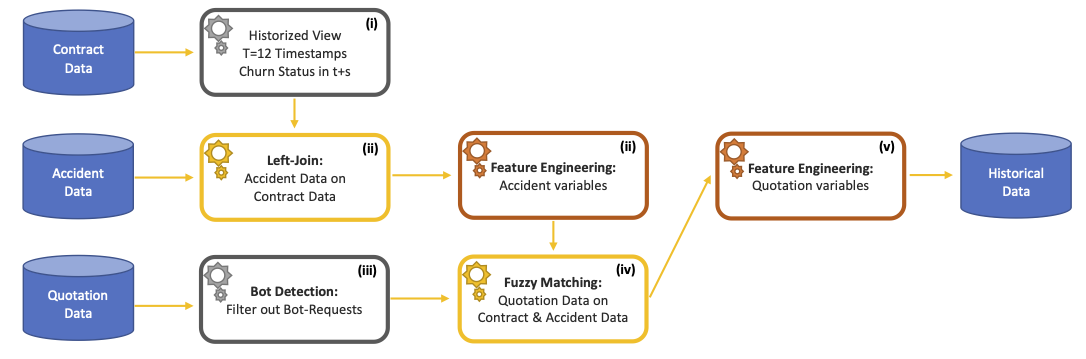
\includegraphics[height=6cm]{data_preparation.png}}
\caption{Vizualization of Data Preparation}
\label{fig:preparation}
\end{figure}

\subsubsection*{(i) Creating the historized view of the Contracts}
As already mentioned, the source table containing all contract information is a VTST. So any desired point in time $t$ in the past can be selected to collect all active contracts to that time. We use $T=12$ points in time in the past, following the findings of Gattermann-Itschert et al. \cite{multiplets}, to ensure a larger dataset and higher generalizability and robustness over time. So in the first step we generate 12 different tables, which are essantially views on the source table for the given points in time.\\
For each generated view-table (for each point in time $t$) and for each active contract we look for the status of that contract in $t+s$. This is done by joining the same table filtered for timestamp $t+s$ on the unique identifier column "contract\_number". To ensure we only collect mid-contract-churns, we check if the termination date of that contract is unequal to the agreed upon termination date. The case where both dates are equal is excluded in our modelling question and therefore not seen as a churn. \\
The 12 points in time are selected carefully, in a sense that there is no overlapping between any time window $(t, t+s]$. So following property must hold for any pair of time sets: $(p, p+s] \cap (q, q+s] = \emptyset$ for all $p \neq q$ and $p,q=1,...,12$. \\
The final step for generating a historized view of the contracts is to create a union on all 12 subviews, creating a panel-dataset. The number of resulting rows after this operation equals the number of rows after all next steps. So we have already generated the framework of the prepared table. The only thing which is left is to generate more variables, espacially accident and quotation variables. \\

\subsubsection*{(ii) Join accident data}
In many modelling problems in the insurance context it turns out that the driving behavior of the customer plays a big role in predicting the desired outcome. Espacially in risk modelling, knowing how many times a customer was involved in an accident or how costly these accidents were, ensures good predictions. \\
Being involved in an accident is one of the events which give a customer the exceptional right of terminating the contract. Therefore we also include historized accident data to generate explanatory accident variables. The VTST containing the historized accidents are recorded for each "contract\_number", which makes it easy to join the data to the table generated in (i). \\
We engineer two new variables based on the accident data. One is a simple count of accident the contract holder was involved in since the start of the contract ("n\_accident"). The second one is the sum over the incurred costs corresponding to the accidents ("sum\_accident\_cost"). This quantifies the accidents and makes them comparable. \\


\subsubsection*{(iii) Bot Detection in Quotation Data}

One big issue arises with the usage of quotation data. Not all requests in online distribution channels are generated by humans. The pricing information of a company is valuable for competitors' pricing strategy or other third party institutions. As a result many bots or crawlers are designed to automatically extract data from websites. The proportion of not-human requests can be very high and reaches up to 70\% in one of the distribution channels. \\
As we do not want to consider bots and crawlers and falsely join them as requests from our active customers we need to find a way to detect them. The first best strategy would be to label a proportion of requests as $BOT=True$ or $BOT=False$ and then train a model to estimate $P(BOT=TRUE \mid X)$ for the remaining requests. This however is infeasible as there is no information on the true labeling for any request. \\
The second best approach flags requests with unreasonably high number of same occurences and is used in this work. Thus, it counts the number of requests with the same combination of certain quotation variables (1) over a day and (2) over the entire timeframe. These variables for flagging bots or crawlers should be as unique as possible in a sense that requests coming from the same source are only counted. For both (1) and (2) individually, a certain cutoff percentile of the combinations is specified. A request is then specified as a bot if the rank of its specific combination is larger than the cutoff. \\
The cutoff percentile is defined for every distribution channel individually (as some are more prone for bots than others). How to choose the correct cutoff is done through eyeballing the smoothness of distributions for suitable quotation variables. An example is the variable "time\_of\_day", where we have an expected distribution and can detect anomalies with our eye. \\
Figure \label{fig:bots} illustrates the result of the bot detection algorithm and the distribution of "time\_of\_day" over the entire time since 2018 for one specific online distribution channel. It is a screenshot of the dashboard which is used to monitor the performance of the algortihm. It was also used to finetune the cutoffs for every distribution channel and to choose the right combination of variables. The spikes between 2:30 am and 4:30 am clearly represent such an anomaly and are fully captured by our bot detection algorithm. \\
\begin{figure}[H]
    \centerline{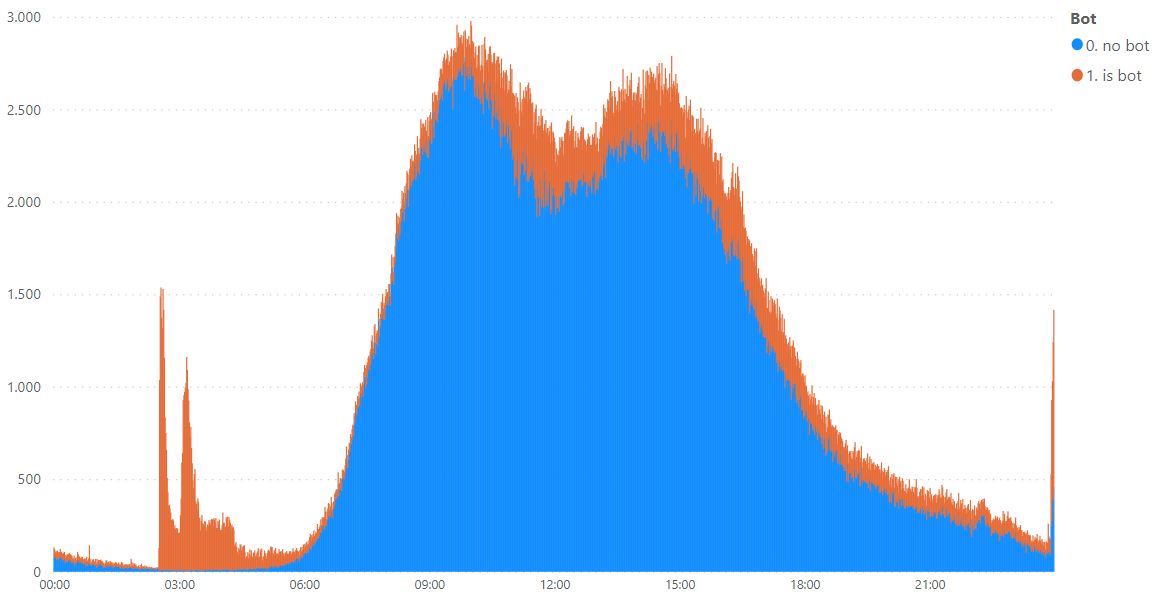
\includegraphics[height=8cm]{bots_day_time.png}}
\caption{Bot Detection Results using "time\_of\_day" as an example}
\label{fig:bots}
\end{figure}
\noindent
The advantage of this algorithm is that it also captures newly arriving bots by calculating percentiles per day. Also it is able to treat the distribution channels individually. The algorithm parameters are easily adjustable and the performance is monitorable. It however still fails to capture certain types of bots which are programmed to enter a different combination of variables in each request. There however, it is nearly infeasible to detect them with any advanced method. In this work we estimate that these bots only make up a very small fraction of the requests and therefore we neglect them. \\

\subsubsection*{(iv) Matching quotation with contract data}
Another issue with the quotation data is that there is no unique identifier column which can be used to correctly join it to the table generated in (i) and (ii). Additionally, columns like "name" or "birthdate" are not always correctly specified during their price request which makes the matching even more difficult. If specified correctly in the quotation data, a combination of these variables could be used as key columns. \\
In order to adress this $M\times N$-Matching problem we need to come up with a fuzzy-matching algorithm. On one side we have a table which contains contracts at different timestamps, their status 2 months later and historic accident information. At the other side we have an ungrouped and unstructured table which simply lists all requests and their corresponding request information. The end result should be of the same structure as the base table created in (i) and (ii) but simply appended with the variables generated from quotation data. We can already expect, that not all contracts have quotation activity $m$ months before $t$. Also, not every request is associated with a contract holder. These two facts increase the uncertainty of matching but are necessary to check the scope and quality of matching. \\
The main idea behind our fuzzy-matching algorithm is to try to match both tables with a different set of signals iteratively. Each signal is a collection of variables which together serve as almost unique identifiers. One example for a signal is the combination of the variables: "hsn" (manufracturer key number), "tsn" (type key number), "plz" (postal code) and "birthdate". \\
As we join the quotation table on the contract table multiple times with different sets of signals we expect and first allow for duplicates of same "contract\_id" $\times$ "timestamp" combinations and/or requests. Therefore the next important step in this section is the deduplication. We know that first the combination of "contract\_id" $\times$ "timestamp" and second request\_id should be unique in the end table. \\
The first step of deduplication is to only include requests for each contract, which occured in the corresponding request window $[t-m,t)$. \\
The matching algorithm is designed in a way that it implicitly allows to formulate preferences about the matching signals. So to each signal a preference rank is associated. This is used for the second step of deduplication. To further eliminate duplicates, we only keep the most preferred match per "contract\_id" $\times$ "timestamp" combination on the one hand and per "request\_id" on the other. \\
After the second deduplication step there might still be unwanted duplicates if for example the same requests are joined to different contracts with the same signal preference. To address this last issue we pick the request-contract pair with the smallest time difference. This of course is not always the correct pair, but ensures wrong duplicates. Additionally there is no other information to be exploited for correct matches. Unwanted duplicates occuring after deduplication steps 1 and 2 are however very rare (0.002\%) and therefore can be neglected. \\

Like for the bot detection we generate a dashboard to monitor the quality of the matching algorithm. We have developped three checks which are automatically executed everytime the data preparation is performed. We present them shortly in the following. \\
For all the checks we exploit the fact that every new-business contract, so a newly closed deal between customer and insurance, needs a corresponding request in the quotation data. Therefore we use the same matching algorithm, but instead of joining the quotation data on our base contract table from (i) and (ii) we join it on a new-business table, which is also given in our database. With a perfect matching algorithm we would expect a match rate of 100\%. While monitoring our algorithm a match rate of 100\% should however be regarded critcially as it might be a result of too weak signals. \\
The first check is done by eyeballing the aggregated match-rate of the new-business-contracts over time. In the graph of figure \ref{fig:matchrate} the x-axis represents the starting date of the new-business contracts and the y-axis the match rate to these contracts. The graph shows that the performance of the algorithm is stable and accurate as in the entire time window for over 90\% of the contracts the corresponding request is found. The drop after November 2021 should not be misinterpreted as the plot was generated in November 2021. \\
\begin{figure}[H]
    \centerline{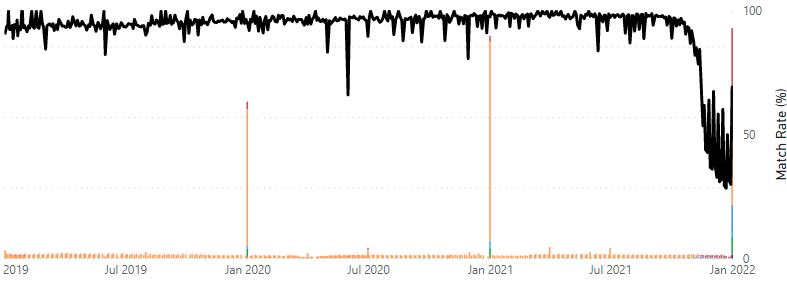
\includegraphics[height=6cm]{matching.png}}
\caption{Match Rate; Evaluation of Fuzzy Matching}
\label{fig:matchrate}
\end{figure}
\noindent
To also ensure the correctness of the matches we monitor the quality by comparing the price determined in the new-business contract with the price of the matched request. Prices are not used in any matching signal for two reasons. One is the fact that after a converted request there may occur specific rebates or other changes to the price which lead to differences between contract price and request price. The second reason is to have an unbiased check of the matching-quality. \\
The resulting second check is generated with the visual in figure \ref{fig:matchquality} where the percentage deviation between contract price and request price are binned into buckets for all new-business contracts. We expect some deviation around plus and minus 20\% for given reasons. Abnormal differences over the 20\% mark indicate a bad match. \\
\begin{figure}[H]
    \centerline{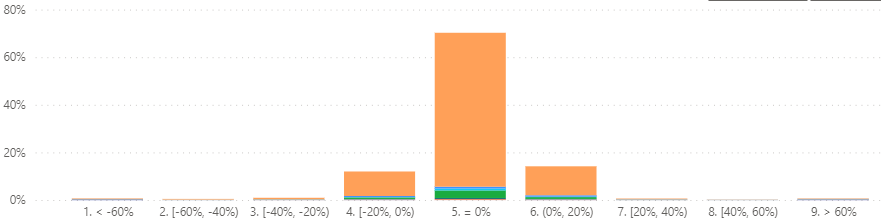
\includegraphics[height=4.3cm]{quality.png}}
\caption{Match Quality; Evaluation of Fuzzy Matching}
\label{fig:matchquality}
\end{figure}
\noindent
As we can see, after optimizing the matching signals and preferences bad matches occur in only a very small proportion. Additionally we can safely say that a minimum of 70\% of the contracts are correctly matched with its request as prices are exactly equal in these cases. Adding the expected deviation of contract and request price we are left with a good quality of matching.\\
The third check also uses the new-business contracts as a test table for the performance of the algorithm. The idea behind this check is however to ensure that the current implementation is the best possible with the underlying data. \\
We therefore model the match status (boolean) of the new-business contract as target variable and all underlying quotation and contract variables as explanatory variables. The model itself is a decision tree. The defining rule to decide wether the algorithm is using the most out of the given information is the resulting variable importance score. More specifically we use the score which assigns its overall contribution to loss reduction to each variable. So for each variable we calculate the decrease in node impurity weighted by the probability of reaching that node.\\
Under full exploitation of the information at hand the decision tree should not be able to find a structure to model the match boolean. In result we should expect complete randomness in the structure of the tree and almost equal variable importance scores for all the variables. If there is any variable with abnormal high variable importance it is a sign for incomplete information usage for matching. \\

\subsubsection*{(v) Generating quotation variables}
The last step of data preparation involves the feature engineering of quotation variables. The variables we generate can be summarized into four groups: \\

\noindent
\textit{(1) n\_requests\_m$_{t - m, t}$:} To each active contract we calculate the number of requests generated by the corresponding customer in the $m$ months before the selected timestamp $t$. We allow for multiple values of $m$, more specifically $m \in \{ 1, 2, 3\}$, resulting in 3 different generated variables for this group. \\

\noindent
\textit{(2) diff\_n\_requests\_m$_{t - m, t}$:} We also calculate the average monthly number of requests in the last $m$ months subtracted by the average monthly number of requests in the last 12 months. The idea behind this group of variables is that it reflects if there is a difference in request behavior of the last $m$ months to the normal behavior. So \textit{diff\_n\_requests\_m$_{t - m, t}$} can be seen as a normalized version (using customer specific averages) of \textit{n\_requests\_m$_{t - m, t}$}. \\

\noindent
\textit{(3) diff\_avg\_vjnbe\_requests\_m$_{t - m, t}$:} Here we use the average shown price of the requests and subtract it with the price the customer is paying according to his/her active contract. Again, we engineer 3 variables in this group, as $m \in \{ 1, 2, 3\}$. \\

\noindent
\textit{(4) diff\_hsntsn\_requests\_m$_{t - m, t}$:} As customers have to state vehicle specific information during their price request, this information can be compared to the vehicle which is insured in the active contract. Thereby we concentrate on the "hsn" (manufracturer key number) and "tsn" (type key number). The combination of both the "hsn" and "tsn" is a unique identifier for the type of the car. Thus, for this group of variables we create a similarity score between 0 and 1. 0 reflects the case where none of the entered vehicles in the requests equals the "hsn"-"tsn"-combination in the contract and 1 is assigned to full similarity between requested car(s) and insured car. The resulting variables can be an indicator for the occurence of event $N$, i.e. the customer thinking about changing his/her car. \\

\noindent
Note that for each group we generate multiple variables with different values for $m$. Our purpose is to find the optimal request window $m^{\star}$ for each group using a dimension reduction technique called MRMR. This technique is presented in chapter \ref{chap:mrmr} and is designed to optimally filter the variables when expecting correlation among them. This is highly reasonable for our quotation variables.\\

\noindent
To summarize the data preparation we presented the challanges and methods used to generate a modelling-ready data-set. The steps needed to get to this end result are illustrated in figure \ref{fig:preparation}. We are now ready to present modelling related methodologies used in this work. \\

\subsection{Modelling Structure} \par
\label{chap:modstruct}

To avoid overfitting and to ensure reliable and stable results we follow a strict modelling structure for our model approaches. Therefore we split the historical data set into a training (80$\%$), validation (10$\%$) and test set (10$\%$). Thereby the splits are performed in a stratified manner, ensuring approximately the same proportion of churners in all subsets. \\
Every modelling approach involves two sets of hyperparameter (HP) tuning loops. We name the first loop the Structural-HP-Tuning-Loop (S-HPTL). This loop aims to identify the best set of all preprocessing HPs which involves the type of sampling, the type of dimension reduction and the type of objective loss function. The second loop nests in the S-HPTL and involves all model-specific HPs. We name this second loop the Model-HP-Tuning-Loop (M-HPTL). As it nests in S-HPTL, the entire loop of M-HPTL is executed in each iteration of S-HPTL. \\
Additionally, in each iteration of M-HPTL we fit the underlying model using a 3-fold cross-validation on the training set to ensure reliable training scores. The validation set is used for both GBT and EBM to evaluate the performance of the model mid training. After having fitted all the candidates corresponding to the M-HPTL we pick the set of Model-HPs which yields the best evaluation scores. With this set of HPs we fit the underlying model once more, but this time with the entire training set and no cross-validation. This model is used, tested on unseen data and presented as a candidate model for the corresponding set of Structural-HP's of the current iteration of S-HPTL. \\
In a last step we manually compare all best candidates resulting from S-HPTL and pick the set of preprocessing HP's which yield the best evaluation scores. The figure \ref{fig:shptl} illustrates one iteration of the S-HPTL. \\
\begin{figure}[H]
    \centerline{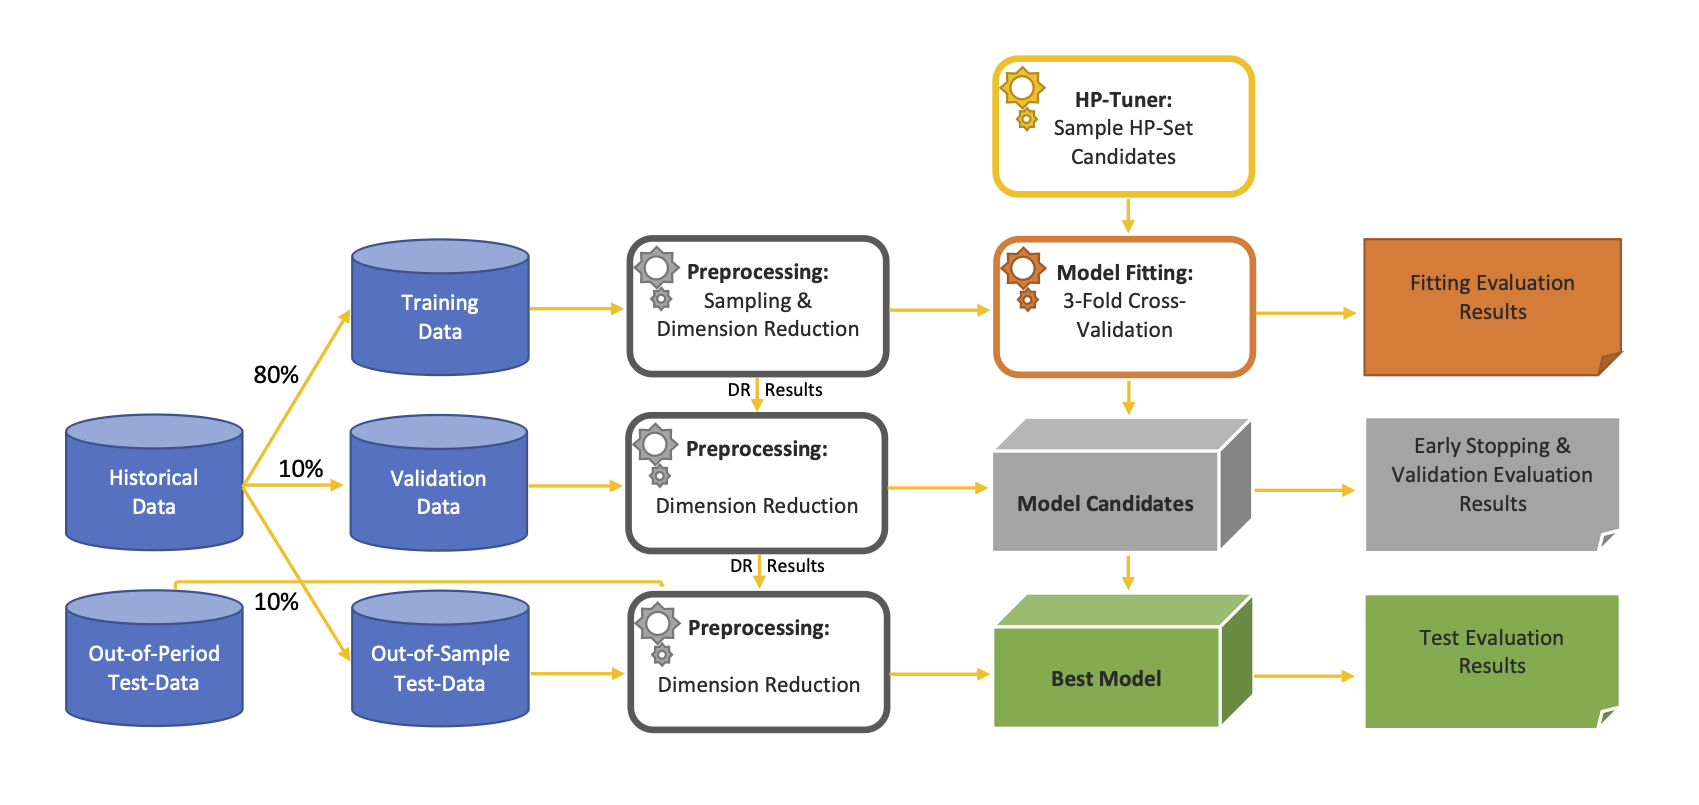
\includegraphics[height=8cm]{fitting_tuning_viz.png}}
\caption{Modelling Structure; One Iteration of S-HPTL}
\label{fig:shptl}
\end{figure}
\noindent
This entire modelling approach is set up as it is to ensure reliable, robust and accurate results for the HPs, parameters, predictions and evaluation metrics. It additionally enables us to compare the different options of dimension reduction, sampling and the objective loss-functions presented in the following subchapters. \\

\subsection{Dimension Reduction} \par
\label{chap:mrmr}

A full collection of the explanatory variables in our data can be found in figure \ref{fig:eda}. As we most of the quotation variables we generate are highly correlated, preprocessing this data set is essential. The goal is to retain only the minimal optimal subset of quotation variables. In many cases, due to multicollinearity in models with many variables, dimension reduction techniques can even improve the predictive performance of models. \\
In the current literature of machine learning there are many approaches for variable selection, ranging from manual selection to fully automated selection procedures. We use the "Maximum Relevance Minimum Redundancy" (MRMR) - approach designed by Ubers machine-learning researchers Zhao et al. \cite{mrmr}. The authors focus on designing an algorithm which detects the best subset of instead of the subset of best variables. The latter is often used in applications of machine learning, where a model is trained and the selection is performed a posteriori based on certain importance scores for that model. This however does not eliminate redundant variables, which in reality do not improve the model performance due to being already represented in correlated other inputs. \\
Using the best subset also helps us to identify the optimal length of the request window $m$ per quotation variable group. As we want to examine the impact of quotation data for predicting customer churn, we include multiple number-of-request variables with different values for $m$ in our unfiltered selection of variables $F$. These are obviously expected to be highly correlated, which additionally delivers a possibility to monitor the effectiveness of the MRMR. \\
MRMR works iteratively, so at each iteration a new best variable is identified and added to the list of selected variables. Once a variable is selected it can not ever be unselected in the next iterations. One drawback of this approach is that the number of iterations and therefore the number of selected variables has to be predefined. We extend it however in a way that we iterate through the entire variable set $F$ and cache the resulting sets and scores of each iteration. So the resulting iterative process starts with an empty selected $S$ and full unselected $U$ set and ends with a full $S$ and an empty $U$. This lets us define the optimal number of iterations retroactively. \\
The algorithm MRMR got his name from the fact, that at each iteration $j$ a new variable is selected into $S$ that has the maximum relevance with respect to the target variable scaled by the redundancy with respect to the variables that are already in $S$. Therefore at each iteration and for each of the remaining variables in $U$ the following score is computed:
\vspace{5mm}
\noindent
\begin{equation} \label{score_raw}
    score_{i}(variable_{i \in U}) = \frac{rel(variable_{i \in U}, C)}{red(variable_{i \in U}, variables \in S)} \\
\end{equation}
\vspace{1mm}

\noindent
The sets $U$ and $S$ get updated each iteration by transfering the variable with the highest score from $U$ to $S$. In their paper, Zhao et al. present multiple metrics for both relevance and redundancy. We focus on one approach which yields the best result in their paper. \\
At each iteration the relevance of the remaining variables in $U$ has to be computed with a new model utilizing only these remaining variables. We use gradient boosted trees and its package "lightgbm" (LGBM) in python in each iteration to score the new relevance of each remaining variable. LGBM has a build in method for calculating variable importance which is used in this MRMR-setting to represent relevance of a variable. There, variable importance is computed as the number of times that specific variable is selected for a split. How gradient boosted trees work is explained in chapter \ref{chap:mlmodels}. \\
For redundancy an average over certain standardized metrics for the relationship between the to be evaluated variable and the variables already in $S$ needs to be computed. These metrics depend on the scales of measurement for the variables. Zhao et al. only cover the case of continuous variables and their relationship. We extend the redundancy score to categorical and binary variables. Thereby we pay attention to the fact, that the scores need to stay comparable for the different scales. Therefore the chosen metrics (see \cite{correlation}) are all standardized to values between 0 and 1, where 0 indicates no and 1 the strongest possible relationship. The different scale pairs and their relationship metrics can be summarized by table \ref{redtable} (Cramers-V-Correlation: C.-V-Correlation, Point-Biserial-Correlation: P.-B.-Correlation, Bravais-Pearson-Correlation: B.-P.-Correlation).
\setlength{\tabcolsep}{10pt} % Default value: 6pt
\renewcommand{\arraystretch}{1.2}
\begin{center}
\begin{table}[H]
    \begin{tabular}{|l|lll|}
    \hline
     & nominal & binary & continuous      \\
    \hline
    nominal                & C.-V-Correlation &         &                 \\
    binary            & C.-V-Correlation & C.-V-Correlation &                 \\
    continuous             & Eta-Correlation & P.-B.-Correlation & B.-P.-Correlation \\
    \hline
    \end{tabular}
    \caption{Relationship Metric based on Scale}
\label{redtable}
\end{table}
\end{center}
\noindent
Redundancy is then calculated by the mean of the relationship scores as follows:
\vspace{5mm}
\noindent
\begin{equation} \label{redundancy}
    red(variable_{i \in U}, variables \in S) = \frac{1}{n(S)} \mathlarger{\sum}_{s=1}^{n(S)} relationship(i, s)
\end{equation}
\vspace{1mm}

\noindent
The slightly modified MRMR-approach we use can therefore be illustrated by this simplified pseudo-code: \\
\begin{algorithm}[H]
\caption{MRMR-Algortihm}\label{alg:mrmr}
\begin{algorithmic}
    \State $corrmatrix \gets corr(X)$
    \State $S \gets \left[ \right]$
    \State $U \gets \left[X.columns\right]$
    \State $cachedict \gets \{\}$
    \For{j in range len(X.columns)}
        \State $relvector \gets LGBMscorer(U)$
        \State $redvector \gets mean(corrmatrix\left[U\right]\left[S\right])$
        \State $scorevector \gets relvector/redvector$
        \State $bestfeat \gets max(scorevector).name$
        \State $bestscore \gets max(scorevector)$
        \State $S.append(bestfeat)$
        \State $U.drop(bestfeat)$
        \State $cachedict.append(j,bestfeat, bestscore)$
    \EndFor
\end{algorithmic}
\end{algorithm}
\vspace{1mm}

As the type of dimension reduction is part of the S-HPTL, we use two different sets of explanatory variables as the sets of HP's. One set uses the best set of quotation variables as a result of MRMR. The other set exludes all quotation variables in order to indicate and evaluate the predictive power of quotation data. \\

\subsection{Handling Class Imbalance} \par

Studying the rarity of an event in the context of machine learning has become an important challange in the recent two decades. Rare events, such as a customer churning in the next period, are much harder to identify and learn for most of the models. HaiYing Wang et al. \cite{convergence_rareevents} study the convergence rate and distributaional properties of a Maximum-Likelihood estimator for the parameters of a logistic regression while predicting rare events. Their finding is that the convergence rate of the MLE is equal to the inverse of the number of samples in the minority class rather then the overall size of the training data set. So the accuracy of the estimates for the parameters is limited to the available information on the minority class, even if the size of the dataset is massive. \\
Therefore some methods have been developed to decrease the problematic of imballanced classes. In this chapter we present different methods which can be applied to the training set, before feeding it to the model. Also, we present different objective loss functions which also aim in solving the problematic. To handle and evaluate the outcomes
of predicting rare events also the appropriate models and model evaluation metrics must be chosen. This is discussed in the next two subsections however. \\

\subsubsection*{(i) Downsampling}

The first basic sampling method is named downsampling. It randomly eliminates samples from the majority class in order to artificially decrease the imballance between the two classes. The downside of this approach is that it possibly eliminates useful samples for the model to maintain a high accuracy in predicting the majority class \cite{mining_rarity}. HaiYing Wang et al. also study the convergence rate and distributional properties when applying downsampling. According to their findings the asymptotic distribution of the resulting parameters may be identical to the MLE's using the full data set. Under this condition there is no loss in terms of efficiency (minimum possible variance of an unbiased estimator devided by its actual variance). \\

\subsubsection*{(ii) Upsampling}

The second basic sampling method is the upsampling approach. This method simply duplicates samples from the minority class to reach a higher balance. While duplicating samples though, the chances of overfitting to these duplicates becomes a more probable threat. Also, no new data is being generated in order to let the model learn more valuable variables about the minority class \cite{mining_rarity}. Additionally, the computational performance of this approach can get rather poor, espacially with large datasets and highly imballanced classes. While evaluating the asymptotics of the MLE's with upsampling, HaiYing Wang et al. find out that it also decreases the efficiency. A probable higher asymptotic variance of the estimators is the reason for that. \\

\subsubsection*{(iii) SMOTE}

The more advanced SMOTE-approach (Synthetic Minority Oversampling Technique) \cite{smote} also creates more artificial samples of the minority class. Instead of simply duplicating some rows SMOTE creates new nearest neighbors in terms of variable values for the minority class samples. While constructing the variable values of the new sample $(N + 1)$ as a new nearest neighbor for sample $i$ one has to differentiate between continuous and nominal variables. The k-nearest neighbors for the minority class are typically constructed with the Euclidean Distance for continuous variables and the Value Distance Metric for nominal variables. The structure of one new-sample-creation for both types of data is presented in the next two paragraphs.
\vspace{6mm}
\indent

\textbf{A} Continuous variables: \\
1) Construct difference between corresponding variable value of sample $i$ and one of its k nearest neighbors. \\
2) Multiply this difference with a random value drawn from a uniform distribution between 0 and 1. \\
3) Construct the variable value of the new sample by adding the multiplied difference to the variable value of sample $i$.
\vspace{6mm}
\indent

\textbf{B} Nominal variables: \\
1) Choose the variable value which is the majority vote between the variable value $i$ and its k nearest neighbors. \\
2) Assign this value to the corresponding variable of the new sample.
\vspace{6mm}

\noindent
With this approach it is ensured that the model learns more about the neighborhood regions of the minority class. It decreases the probability, that the model overfits to the duplicates created in upsampling. The drawback of this approach however is that the computational time is even higher than with simple upsampling. Also, the new samples do not reflect real information and might therefore also lead to out-of-sample accuracy losses. The literature agrees on SMOTE's effectiveness is application dependent \cite{mining_rarity}. \\

\subsubsection*{(iv) Cost-Sensitive Classifiers} \label{Cost-Sensitive Classifiers}
One disadvantage of the up-to-now presented sampling methods is the need to change the data distribution. A different starting point is to alter the objective loss function which is minimized during the model fitting. Thereby the data size and the distribution stay the same. In the modified cost function we want to penalize false-negative
classifications with a higher weight. Reason behind this is to ensure that the event of interest, represented by the minority class, is predicted correctly \cite{cost_sensitive}. \\
The challange of this approach is to find the appropriate penalty parameters. It is hard to measure the cost of misclassifying an insurance-customer regarding churn-probabilities. The fact that these costs can come from multiple sources which are not easily definable is one part of the reasoning. Therefore we focus on two types of custom loss functions.\\
One conventional method is to assign simple parameter weights $\alpha$ and $1 - \alpha$ to the loss function. By default one might use the inverse of the class frequency as the associated weights. These parameters however can also be optimized during the structural HP-tuning loop. We call this method the "Simple Weighted Loss Function". The derivation is part of the next subchapter.\\
The second approach is called "Focal Loss Function" and was originally designed by FAIR (Facebook Artificial Intelligence Research) for an object detection purpose \cite{focal}. As it also aims to penalize false-negative classifications it is widely used for predicting rare events. Again, the exact structure of the modified loss-function is shown in the next subchapter and the parameters are tuned with the S-HPTL.
\vspace{6mm}

\noindent
To conclude we present 3 sampling methods and two cost-sensitive loss functions. For our S-HPTL, we allow for a combination of both sampling and cost-sensitive learning at the same time, as they do not exclude each other. \\


\subsection{Machine Learning Models} \par
\label{chap:mlmodels}

In this section we present and explain mathematical and statistical theoretics behind the machine learning approaches used to model churn in this work. As already stated, the two modelling approaches in this work are gradient boosted trees (GBT) and explainable boosting machines (EBM). GBT are selected due to its known predictive accuracy on tabular data. We compare it to EBM, which essantially aims to provide an explainable model structure. \\
In order to provide the mathematical and statistical intuition behind GBT and EBM, less complex models have to be explained first as they build upon them. That is why we start with logistic regression and classification trees and work our way up to the more complex models. \\

\subsubsection*{(i) Logisitic Regression}
The logistic regression is used as a benchmark model for all classification problems. It has high advantages in terms of computational complexity and interpretability, but fails in capturing complex relationships and interactions. As it has the lowest accuracy of all classifiers it is mostly used as a baseline model in order to evaluate the advantages of additional complexity in the models, as in GBT and EBM. We however use a different baseline in our modelling approach and therefore only introduce it as the logic is needed for the more complex models.\\
Logisitic regression applies a sigmoid function to the linear regression model in order to get output values (probabilities) between $0$ and $1$ as in a Bernoulli distribution. We use the following conventional notation throughout this work:
\vspace{5mm}
\noindent
\begin{equation} \label{bern_dist}
    \hat{C}_{\{t+s\}} = P(C_{\{t+s\}}=1\mid X_{\{t\}}) = f\big(g(X_{\{t\}})\big) = \frac{e^{g(X_{\{t\}})}}{1 + e^{g(X_{\{t\}})}} \\
\end{equation}
\vspace{1mm}

\noindent
Note that from now on we use a vectorized notation. So $\hat{C}_{\{t+s\}}$ represents a vector of probabilities $(\hat{C}_{1,\{t+s\}}\:\hat{C}_{1,\{t+s\}}\:...\:\hat{C}_{N,\{t+s\}})$. The i'th element ($i = 1,...,N$) corresponds to the probability of contract i churning in time $t+s$. This probability vector is constructed by a model conditional on a variable matrix $X$ at time $t$. Again, each row of $X$ represents a different contract and column j is variable j ($j = 1,...,M$). \\
Therefore $f(\cdot)$ is the sigmoid function used on function $g(\cdot)$, where in logistic regression $g(\cdot)$ is a linear model. For GBM and EBM this function is allowed to be more complex.
\vspace{5mm}
\noindent
\begin{equation} \label{lin_model}
    g(X_{\{t\}}) = \beta X_{\{t\}} + \epsilon_{\{t\}} \\
\end{equation}
\vspace{1mm}

\noindent
As the classification models output probabilities between 0 and 1 for a churn, a cutoff $\tau$ is needed in order to create assignments to each class. The rule of thumb is to set $\tau = 0.5$, such that probabilities larger than $0.5$ are predicted as churns and the rest as non-churns. We see that the optimal $\tau$ is application dependent and relies on the type of sampling and loss function which is tried to be minimized. Typically a high $\tau$ ensures, that a high percentage of positive classified samples are in fact positive. A lower $\tau$ however ensures that a higher amount of churners are detected (but with lower precision).
\vspace{5mm}
\noindent
\begin{equation} \label{tau}
    \hat{C}_{\{t+s\}}^{class} = \begin{cases}
        1,& \hat{C}_{\{t+s\}} \geq \tau \\
        0,& \hat{C}_{\{t+s\}} < \tau
    \end{cases}
\end{equation}
\vspace{1mm}

\noindent
We apply Maximum Likelihood to estimate the vector of parameters $\beta$ of the model. It maximizes the joint probability that the status of the contracts are drawn from the Bernoulli distribution stated in equation (\ref{bern_dist}). For the final model in production, when estimating probabilities for a churn in the next period, $t$ is of course equal across all contracts in $X$. But as already stated, when it comes to training the model we use multiple timestamps of the historized data. \\
For the training part of this work we therefore leave out the index $t$ in order to avoid a misleading notation. $N^{train,k}$ corresponds to the number of samples in the k-th ($k=1, 2, 3$) fold of the training data. As the model is retrained on the entire training set after cross-validation, $N^{train,full}$ samples are used in the equations below. We will generalize the notation with $N^{train}$ which corresponds to $N^{train,k}$ during cross-validation and to $N^{train,full}$ during refitting. Still, the status of contract $i$ is determined after $s$ units of time for all contracts. The likelihood function to be maximized during training is described as follows:
\vspace{5mm}
\noindent
\begin{equation} \label{logistic_MLE}
    \mathcal{L}(C; X, \beta) = \prod_{i=1}^{N^{train}}P\big(C_{i}=1\mid X_{i}\big)^{I(C_{i}=1)}\Big(1 - P\big(C_{i}=1\mid X_{i}\big)^{1 - I(C_{i}=1)}\Big) \\
\end{equation}
\vspace{1mm}

\noindent
To describe this term as a loss function it is characterized by the negative logarithm of equation (\ref{logistic_MLE}), which can be minimized with respect to $\beta$ using Gradient Descent, Newton Raphson or other optimization methods.
\vspace{5mm}
\noindent
\begin{equ}[!ht]
\caption{\textbf{Log Loss Function}}
\begin{equation} \label{logistic_log_MLE}
    \begin{aligned}
        l(C; X, \beta) & = -\mathlarger{\sum}_{i=1}^{N^{train}}C_{i}\log\big(P(C_{i}=1\mid X_{i})\big) + (1 - C_{i})\log\big(1 - P(C_{i}=1\mid  X_{i})\big) \\
        & = -\mathlarger{\sum}_{i=1}^{N^{train}}C_{i}\log(\hat{C}_{i}) + (1 - C_{i})\log(1 - \hat{C}_{i}) \\
    \end{aligned}
\end{equation}
\end{equ}
\vspace{1mm}

\noindent
In applications with high dimensional data it makes sense to add a penalty term to the loss function to avoid overfitting during training. While minimizing the loss function, this additional penalty term either shrinks some parameters of $\beta$ towards zero (L2 regularization), or sets some to exact 0 (L1 regularization). However, we can also reduce the dimension of variables prior to fitting the model, as already explained with the MRMR-approach. \\

As already mentioned in chapter \ref{Cost-Sensitive Classifiers}, one technique to handle imbalanced classes is to use cost-sensitive loss functions. We can implement this by setting additional penalty weights to our loss function. The resulting objective "Simple Weighted Loss Function" is described as:\\
\vspace{5mm}
\noindent
\begin{equ}[!ht]
\caption{\textbf{Simple Weighted Loss Function}}
\begin{equation} \label{loss_fct_wl}
    l(C, \hat{C}) = -\mathlarger{\sum}_{i=1}^{N^{train}}\alpha C_{i}\log(\hat{C}_{i}) + (1-\alpha)(1 - C_{i})\log(1 - \hat{C}_{i})
\end{equation}
\end{equ}
\vspace{1mm}

\noindent
The additional parameter of $\alpha$ is a hyperparameters which can be tuned during S-HPTL. Following Gattermann Itschert et al. \cite{multiplets} approach, $\alpha$ can also be set by default to the inverse of the relative class frequency of the majority class in the training data. \\
To provide further intuition behind the idea of using a weighted loss function we look at the individual loss for different values of $\alpha$. For $\alpha>0.5$ we reach the desired state of penalizing false-negative classifications more than false-positive ones. To see why this is the case it is best to look at the single log-loss for a positive sample. Positive samples in equation (\ref{loss_fct_wl}) can be seen as the insertion of $C_{i}=1$ which simplifies the individual loss to $-\alpha \log(\hat{C}_{i})$. For higher $\alpha$, the loss gets higher for every $\hat{C}_{i}$. This example is vizualized by the following plot: \\
\begin{figure}[H]
    \centerline{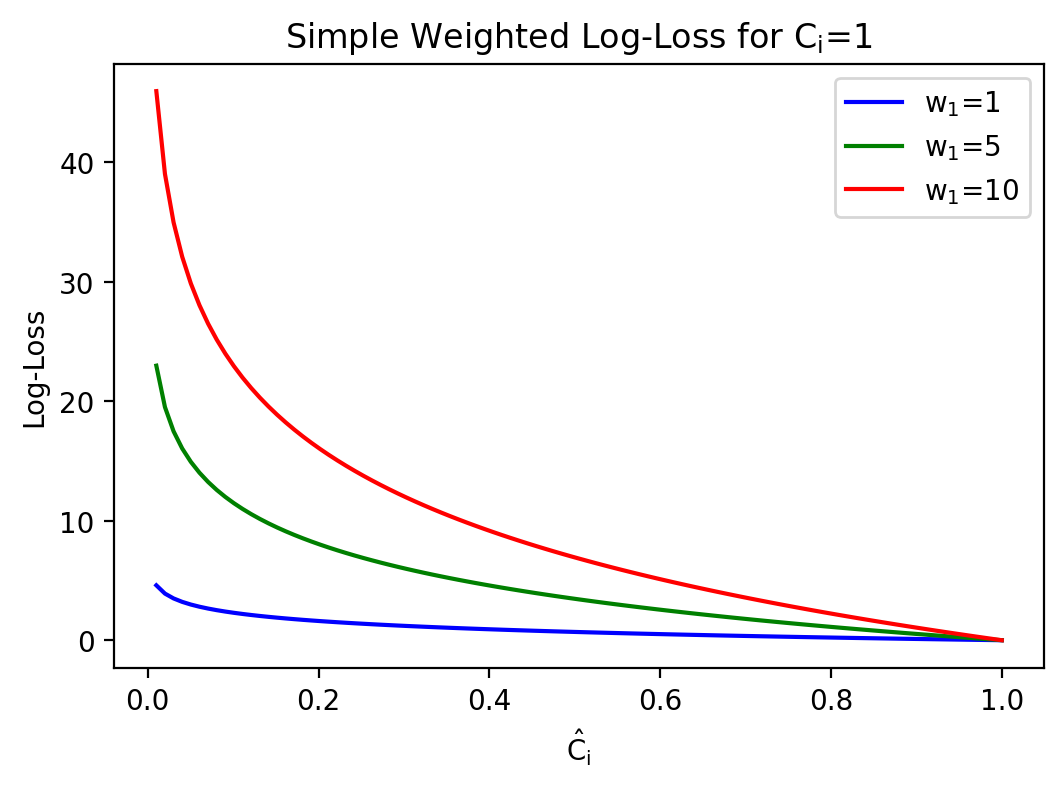
\includegraphics[height=8cm]{weighted_loss.png}}
\end{figure}
\noindent
This can be done analogously for negative samples. The individual loss for $C_{i}=0$ simplifies to $-(1-\alpha)\log(1-\hat{C}_{i})$. We therefore see that for $\alpha>0.5$ the relative penalty for false-negative classifications is higher than for false-positives. \\

Going one step further and introducing one more adjustable parameter to the objective function we arrive at the "Focal Loss Function". It is structured as in equation (\ref{loss_fct_fl}). \\
\noindent
\begin{equ}[!ht]
\caption{\textbf{Focal Loss Function}}
\begin{equation} \label{loss_fct_fl}
    l(C, \hat{C}) = -\mathlarger{\sum}_{i=1}^{N^{train}}\alpha(1 - \hat{C}_{i})^{\gamma}C_{i}\log(\hat{C}_{i}) + (1 - \alpha)\hat{C}_{i}^{\gamma}(1 - C_{i})\log(1 - \hat{C}_{i})
\end{equation}
\end{equ}
\noindent
Again, $\alpha$ and $\gamma$ are hyperparamaters, which are tuned during S-HPTL. Note that for $\gamma=0$ (\ref{loss_fct_fl}) becomes a "Simple Weighted Loss Function". So the same intuition for varying weights $\alpha$ can be applied here. Also note that for $\gamma=0$ and $\alpha=0.5$ we are left with the original log-loss function derived in equation (\ref{logistic_log_MLE}) multiplied by $0.5$. \\
To understand how $\gamma$ can be used to improve modelling, we again look at the single loss for a positive sample $C_{i}=1$. As $\gamma$ affects the loss for positive and negative classifications analogously, the same logic can be applied for $C_{i}=0$. Thereby we again plot the loss for different values for $\gamma$ and $\hat{C}_{i}$ and set $\alpha=0.5$. \\
\begin{figure}[H]
    \centerline{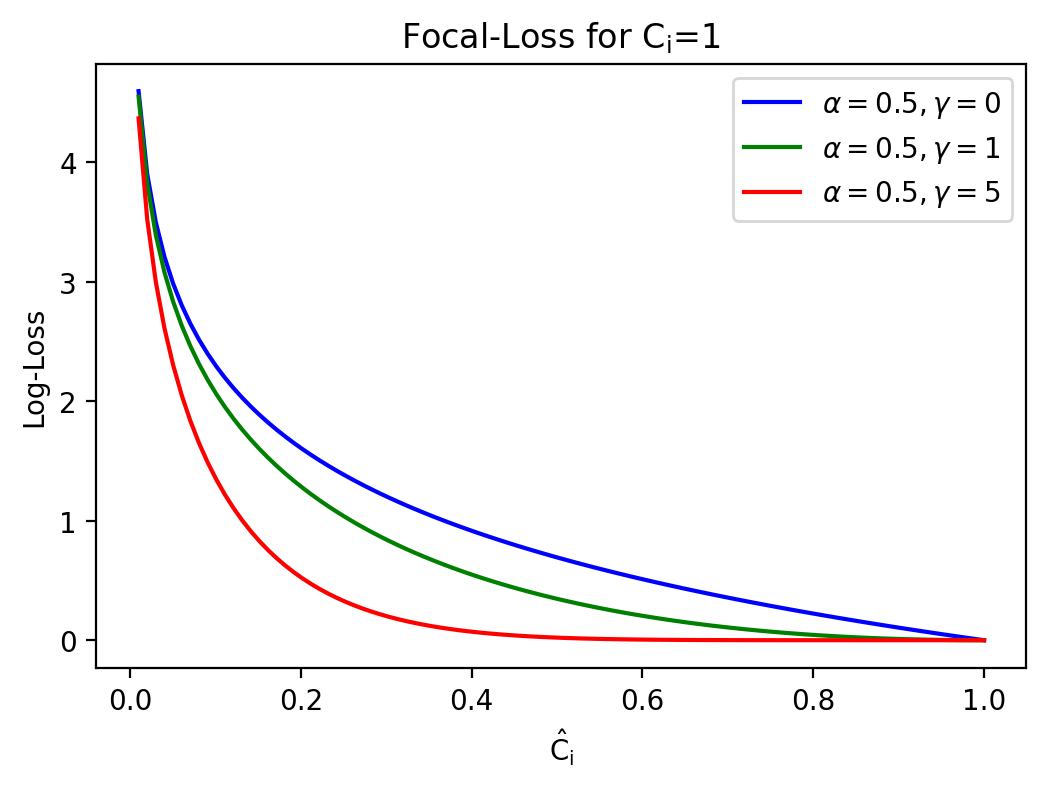
\includegraphics[height=8cm]{focal_loss.png}}
\end{figure}
\noindent
As illustrated a positive $\gamma$ skews the function in a way that small to medium deviations of $\hat{C}_{i}$ from the true $C_{i}$ are not penalized as much as in the normal log-loss function. Strong deviations however are penalized almost as much as in the normal function. This introduces the effect of a higher relative loss for "bad" false classifications. \\
Both equation (\ref{loss_fct_wl}) and (\ref{loss_fct_fl}) aim to tackle the issue of having highly imbalanced classes. We use and compare both with different parameters in the S-HPTL and select the one which performs best on unseen data. \\

\subsubsection*{(ii) Tree-based Classifier}

\vspace{6mm}
\indent

\textbf{A} Single Classification Tree: \\

Classification trees have a different approach on builing a prediction model for $\hat{C}_{t+s} = P(C_{t+s}=1\mid X_{t})$. Unlike linear or logistic regression, they allow for non-linearities and interactions. Classification trees search for the optimal sequential binary sample splits in order to minimize an inner objective loss function. So at each node of the tree the optimal variable $j$ and its optimal split point $r$ need to be found. The search at each node can be formalized as follows:
\vspace{5mm}
\noindent
\begin{equ}[!ht]
\begin{equation} \label{dec_tree}
    \begin{aligned}
        \{j, r\} \in \argmin_{j, r} \mathlarger{\sum}_{i:X_{i}\in S_{1}(j, r)}L(C_{i}; X_{i}, \hat{p}_{k}) + \mathlarger{\sum}_{i:X_{i}\in S_{2}(j, r)}L(C_{i}; X_{i}, \hat{p}_{k}) \\
        \text{with: }S_{1}(j, r) = \{X\mid X^{(j)}\geq r\} \text{, } S_{2}(j, r) = \{X\mid X^{(j)}< r\}
    \end{aligned}
\end{equation}
\end{equ}
\vspace{1mm}

\noindent
The loss function for region $S_{k}$ is calculated using the resulting region prediction $\hat{p}_{k}$. This region prediction is applied to all obeservations which are assigned to it after the splits $i:X_{i}\in S_{k}$). In a classification setting the prediction simplifies to the shares of churns in $S_{k}$. The typical loss functions are based on evaluating the purity of the resulting regions. In the ideal case, one would like to find the splits in $X$ which always correctly assign contracts of the two classes into two different regions. In this case, $\hat{p}_{k}$ would always be either 1 or 0. In order to approach this case one either uses the Gini-index or the Cross-entropy for region $S_{k}$:
\vspace{5mm}
\begin{center}
    \begin{tabular}{ll}
        Gini-index: & $2\hat{p}_{k}(1-\hat{p}_{k})$ \\
        Cross-entropy: & $-\hat{p}_{k}\log(\hat{p}_{k}) - (1-\hat{p}_{k})\log(1-\hat{p}_{k})$ \\
    \end{tabular}
    \label{purity}
\end{center}
\vspace{5mm}
\noindent
The splits at each node are performed until certain criteria for the loss functions or other hyperparamaters are met. Hyperparameters of a single tree are summarized in table 2. To get the prediction $\hat{C}_{i}$, one assigns $\hat{p}_{k}$ as the region prediction of the corresponding end node of observation $i$ to that value. \\
\vspace{6mm}
\indent

\textbf{B} Boosted Trees for Classification: \\

In most applications the predictions of a single classification tree have high variance due to overfitting to the training data. The accuracy in the prediction on unseen data is therefore rather poor compared to the accuracy during training. Random forests \cite{randomforest} are designed to reduce the variance of the predictions, by averaging over predictions of multiple independent trees. This phenomenon is called "Wisdom of the Crowds". It is underlined by the fact that the average of multiple estimators for the same parameter has the same bias but a smaller variance (how much depends on the number of estimators) than a single estimator. \\
The current literature however agrees on the fact that Gradient Boosted Tree Algorithms outperform Random Forests, and therefore also a single tree. Therefore we focus on the core methodology and hyperparameters of boosted trees in the following. \\
The idea of boosted trees for classification is to have a sequence of dependent base learners (trees), which improve in terms of accuracy where it is most needed. Thereby, the base learners $\hat{g}_{b}(X)$ ($b=1,..,B$) are constructed in a shallow shape, avoiding an overfitted single learner. Additionally the trees $\hat{g}_{b}(X)$ are now regression trees, which output values in $(-\infty, \infty)$. So for the optimal split at the nodes of each tree the squared error reduction of the log-odds are now being compared. To get a probability in $[0, 1]$ we again have to apply the sigmoid function $f(\cdot)$. The resulting loss of each tree is then fitted by the preceeding trees. So the procedure can be summarized by this pseudo code: \\

\begin{algorithm}
\caption{GBT-Algortihm}\label{alg:boostedtrees}
\begin{algorithmic}
    \State $\hat{G}(X) \gets 0$
    \State $L \gets \mathlarger{\sum}_{i=1}^{N^{train}} l(C_{i}, f(\hat{G}(X_{i})))$
    \For{b in range(1, B)}
        \State Fit tree $\hat{g}_{b}(X)$ which minimizes $L = \mathlarger{\sum}_{i=1}^{N^{train}} l\Big(C_{i}, f\big(\hat{G}(X_{i}) + \hat{g}_{b}(X_{i})\big)\Big)$
        \State $\hat{G}(X) \gets \hat{G}(X) + \lambda\hat{g}_{b}(X)$
    \EndFor
    \State $\hat{C} = \hat{f}(\hat{G}(X)) = f(\mathlarger{\sum}_{b=1}^{B}\lambda\hat{g}_{b}(X))$
\end{algorithmic}
\end{algorithm}
\vspace{3mm}
\noindent
The hyperparameter $\lambda$ is called learning rate and set to a small number to learn slowly and to avoid overfitting. Also notice, that the loss function defined here is the objective loss function used for gradient boosting. It is different than the inner objective function used for constructing a single tree. We try both custom loss functions for GBT derived in equations (\ref{loss_fct_wl}) and (\ref{loss_fct_fl}) and perform hyperparameter tuning to get the best set of hyperparameters belonging to these loss functions. \\
To apply these custom-loss functions we need to derive the gradient as well as the hessian of this function. Herewith the lightgbm-package \cite{gbt} aims to reduce computation time as it takes the second order taylor expansion to compute the optimal loss minimizing $\hat{f}_{b}(X)$ in each iteration $b=1,...,B$. Gradient and hessian are calculated in the appendix. \\
The main time cost of GBT is learning the single trees, and the most time-consuming part in trees is to find the best split-points. Therefore we make use of the histogram-based approach of the lightgbm-package which aims to tackle this issue. The so called histogram-based approach is designed to bin the variables. This creates high efficiency gains while searching for the optimal splits, especially for continuous variables. \\
Another important aspect to note about lightgbm's implementation of boosted trees is the fact that the base trees grow leaf-wise instead of depth-wise. As proposed by Friedman et al., the idea is to extend nodes in first-best order. Thereby, the best node is the one which maximally reduces the sum of the tree loss function in the resulting regions. This enables the possibility that a first-best split is found at a node in level $r+1$ eventhough in level $r$ only one of two nodes are split. \\
If we let the trees grow without tree structure restrictions to full trees, both the leaf-wise and depth-wise approach result in the same trees. As all gradient boosters rely on shallow trees, the combination of hyperparameters such as the maximum number of leaves, the minimum loss reduction required for a further split the first-best split approach result in a better shallow tree structure. \\
There are a lot of hyperparameters which allow to tune the model structure inside M-HPTL. They can be split into the hyperparameters for single tree structure and hyperparameters for the learning process. In table \ref{hplgbm} is an overview of the hyperparameters we focus on and the corresponding values we use for grid search in M-HPTL. \\
\begin{table}[H]
    \centering
    \begin{tabular}{|c|l|l|}
    \hline
    \multicolumn{1}{|l|}{}                                       & Hyperparameter                            & Grid Search Values       \\
    \hline
    \multirow{4}{*}{\begin{sideways} Boosting \end{sideways}}                         & Boosting learning rate $\lambda$                                                                & Shrinking learning rate  \\
    & Maximum Number of boosted Trees B      &        1000                       \\
    & L1 regularization term on weights      &        $\sim$ [0, 1, 5, 10, 100]         \\
    & L2 regularization term on weights      &        $\sim$ [0, 1, 5, 10, 100]         \\
    \hline
    \multicolumn{1}{|l|}{\multirow{5}{*}{\begin{sideways} Single Tree \end{sideways}}} & Maximum number of tree leaves          &        $\sim$ U(6, 50)           \\
    \multicolumn{1}{|l|}{}                                       & Minimum loss reduction for split       &         0                 \\
    \multicolumn{1}{|l|}{}                                       & Minimum number of samples in new region   &      $\sim$ U(60, 500)         \\
    \multicolumn{1}{|l|}{}                                              & Subsample ratio of columns for tree    &     $\sim$ U(0.4, 1)         \\
    \multicolumn{1}{|l|}{}                                              & Subsample ratio of data for tree &          $\sim$ U(0.4, 1)            \\
    \hline
    \end{tabular}
    \caption{Hyperparameter sets for M-HPTL - GBT}
\label{hplgbm}
\end{table}
\noindent
We make use of an early stopping criterium evaluated on the validation set. It terminates boosting when the loss function does not improve for 30 rounds. \\
So in each iteration and for each model-HP of M-HPTL we randomly sample from the corresponding distribution/set from table \ref{hplgbm}. To ensure generalizable results the current set of HPs in one iteration is evaluated by using cross-validation on the training data. For GBT we sample 100 times from these sets. Multiplying this with the 3-fold fitting, we are left with 300 fits in total resulting from the M-HPTL. The set of model-HPs which yields the best results in terms of evaluation metrics is refitted and selected as a model candidate for the current S-HPTL iteration. \\

Table \ref{shplgbm} summarizes the sets of HP's used for the S-HPTL for GBT. "N" as a hyperparameter for sampling means that no sampling is performed and the length of the training data remains the same. "d" (or "u") downsamples (or upsamples) the data such that both classes have the same number of samples. "dX" (or "uY") samples in a way that the number of samples in the majority (or minority) class is multiplied by $X$ (or $Y$). \\
The normal log-loss function is minimized with the combination of $\alpha$ being "N" and $\gamma$ being "N". For $\alpha$ having assigned a value and $\gamma$ being "N" we optimize the "Simple Weighted Loss Function" defined in equation (\ref{loss_fct_wl}). If both parameters have a value the "Focal Loss Function" from equation (\ref{loss_fct_fl}) is minimized. \\
Additionally, in each iteration of S-HPTL, we run the M-HPTL with two different sets of variables. This is denoted by the row "Variables". More precisely, in each iteration of S-HPTL the best set of quotation variables is determined with MRMR. This is repeated every iteration due to the fact that with different sampling methods, a different set of variables might be optimal. To determine the predictive power of quotation data, we once fit the current M-HPTL with and without quotation variables. \\
\begin{table}[H]
    \centering
    \begin{tabular}{|l|l|}
    \hline
              & Set  \\
    \hline
    Sampling &  [N, d, d0.1, d0.5, u, u10, u50, sm]  \\
    Custom Loss & $\alpha$: [N, 0.6, 0.7, 0.8], $\gamma$: [N, 0.2, 0.5, 1, 2, 5] \\
    Variables & [with\_quot, no\_quot] \\
    \hline
    \end{tabular}
    \caption{Hyperparameter sets for S-HPTL - GBT}
    \label{shplgbm}
\end{table}
\noindent
For the S-HPTL we try out each and every combination of the values in the sets for sampling, $\alpha$, $\gamma$ and variables. This totals $8\times4\times6\times2=384$ iterations for the structural loop. Adding to that the fect that in each iteration 300 models are fitted inside the M-HPTL, we end up with $115,200$ models in total. This of course results in a computational complex task, but ensures the needed comparability and optimal (hyper)parameters. \\

\subsubsection*{(iii) Explainable Boosting Classifiers}

Explainable boosting machines (EBM) were developed by researchers at Microsoft \cite{interpretml} and aim to have high accuracy as most complex models, while maintaning an easy interpretable approach. It is maintained by the functional form which is similar to the standard GAM-Model, developed originally in 1987 by Hastie et al. \cite{gam}: \\
\vspace{5mm}
\noindent
\begin{equ}[H]
\begin{equation} \label{gam}
    g(X) = \beta_{0} + \mathlarger{\sum}_{j=1}^{M} k_{j}(X^{(j)}) + \epsilon \\
\end{equation}
\end{equ}
\vspace{1mm}

\noindent
Thereby $M$ is the number of variables and $k_{j}(\cdot)$ is the so called shape function for variable $j$. In standard GAM-models $k_{j}(\cdot)$ is approximated by scatterplot smoothers. In EBM the approximation for $k_{j}(\cdot)$ is allowed to be calculated by a complex modern learner such as a decision tree or a random forest. \\
As the name of the method already reveals, gradient boosting is applied to improve the preceeding trees in direction of the gradient of the loss function. The main difference to the standard gradient boosting classifier is that no longer one tree fits all variables $\hat{g}_{b}(X)=\hat{g}_{b}(X^{(1)}, ..., X^{(M)})$ in each iteration $b=1,..,B$. Instead in each iteration, the algorithm cycles through all variables to improve the single shape functions $k_{j}(\cdot)$, where it is most needed. By cycling through the variables one at a time and maintaining a low learning rate the variable order does not matter and the potential problem of multicollinearity is reduced. \\
Unfortunetaly there is still a huge gap between standard GAM-models and full complexity models in terms of predictive accuracy, even if we allow for non-linearities in $k_{j}(\cdot)$. Full complexity models, such as gradient boosted trees and deep neural nets, have the advantage of allowing for an arbitrary number of interactions between variables. To allow for pairwise interactions, EBM's make use of the idea of GA$^{2}$M-models developed by Lou et al. \cite{ga2m}. The resulting shape functions $k_{m,n}(X^{m}, X^{n})$, (where $m\neq n$ and $m,n \in \{1,...,M\}$) are still interpretable with a heatmap on the two dimensional $X^{m}, X^{n}$-plane. Also, results from Lou et al. not only show that GA2M-models have a high improvement in accuracy over GAM-models, but also compete with high complexity-models in most applications. \\
\vspace{5mm}
\noindent
\begin{equ}[H]
\begin{equation} \label{ga2m}
    g(X) = \beta_{0} + \mathlarger{\sum} k_{j}(X^{(j)}) + \mathlarger{\sum} k_{m,n}(X^{(m)},X^{(n)}) + \epsilon \\
\end{equation}
\end{equ}
\vspace{1mm}

\noindent
We make use bagging, refered to as "inner bags" in the EBM package. At the time of improving the current loss with one individual variable or interaction it fits multiples trees on subsamples (drawn with replacement) from the training data. These trees are averaged out to create the final update of the iteration. This is proven to increase both predictive performance and interpretability of the shape functions.\\
To further ensure both smoothness of the shape functions and reliable estimates, EBM makes use of an outer bagging process. We refer to the hyperparameter name of its package "outer bags". What it essentially does is it fits individual EBMs on different subsamples of the training data. The final shape functions are an average of the shape functions learned in each outer bag. \\

There are a number of approaches to detect the best set of variable interactions for our model as in \cite{anova_interaction}, \cite{pdf_interaction}, \cite{guide}, \cite{grove}. These methods however are either computationally inefficient or almost even infeasible with high-dimensional data. Therefore we use the "FAST" approach by Lou et al. \cite{ga2m}, which are also available in the EBM-package. \\
FAST's structure is based on a greedy forward stagewise selection strategy. It can be compared to the MRMR in a way that it starts with an empty set of selected pairs and an unselected set containing all possible variable pairs. In each iteration all possible unselected pairs are used seperately to fit the current objective loss function resulting from the additive model including only the already selected pairs. The pair with the highest loss improvement is selected in that iteration. The iteration stops, when the objective loss function stops improving for any other inclusion of a pair. \\
If we assume that we have $M$ variables in our data the amount of possible pairwise interactions equals $\binom{M}{2} = \frac{M(M-1)}{2}$. As a result, calculating the set of interaction functions and fitting all possible new models in each iteration is very time consuming for large $M$. FAST therefore builds the interaction functions more efficiently by defining optimized quadrants in the space of the two variables and taking the mean values of each quadrant. \\
The FAST algorithm is performed for each outer bag. Because there are so many interactions, we end up throwing away all but the top $I$ interactions, where k is the number of interactions specified by the modeller. Ranking of the interactions is made by adding the loss improvement of each interaction over all outer bags. \\

EBM also offers hyperparameters to tune. Table \ref{hpebm} lists them and the value spaces used for finding the optimal hyperparameter set. \\
\begin{table}[H]
    \centering
    \begin{tabular}{|l|l|l|}
    \hline
    \multicolumn{1}{|l|}{}                                       & Hyperparameter                            & Grid Search Values       \\
    \hline
    \multirow{2}{*}{Boosting}                         & Learning rate $\lambda$                                                                & $\sim$ U(0.009, 0.015)  \\
    & Maximum number of rounds            &         5000        \\
    \hline
    \multicolumn{1}{|l|}{\multirow{2}{*}{Single Tree}} & Max number of tree leaves          &  $\sim$ U(2, 5)                        \\
    \multicolumn{1}{|l|}{}                                       & Min number of samples for new leaf   &      $\sim$ U(2, 5)       \\
    \hline
    \multicolumn{1}{|l|}{\multirow{3}{*}{Other}} & Number of interactions          &       $\sim$ U(5, 10)      \\
    \multicolumn{1}{|l|}{}                                       & Number of Outer Bags   &        $\sim$ U(20, 30)   \\
    \multicolumn{1}{|l|}{}                                       & Number of Inner Bags   &       $\sim$ U(20, 30)   \\
    \hline
    \end{tabular}
    \caption{Hyperparameter sets for M-HPTL - EBM}
\label{hpebm}
\end{table}
\vspace{3mm}
\noindent
Like for GBT, we apply an early stopping criterium evaluated on the validation set, which terminates boosting when the loss function does not improve for 30 rounds. \\
Again for EBM, in each iteration and for each model-HP of M-HPTL we randomly sample from the corresponding distribution/set from table \ref{hpebm}. We apply cross-validation on the training data for generalizability. For EBM we only sample 10 times from the presented sets. The authors of EBM suggest, that EBM does not need to be tuned as much as GBT in terms of model-hyperparamaters. In combination with 3-fold cross-validation this totals 30 fits resulting from the M-HPTL. The best set of hyperparamaters and its corresponding fit are presented as a candidate model for the current iteration of S-HPTL.\\

The HP-Sets for the S-HPTL we use for EBM are summarized in table \ref{shpebm}. The same logic for the notations and abbreviations from GBT's table \ref{shplgbm} applies here. As custom-loss functions are not applicable with EBM we only have two sets of HP's for the S-HPTL. \\
\begin{table}[H]
    \centering
    \begin{tabular}{|l|l|}
    \hline
              & Set  \\
    \hline
    Sampling &  [N, d, d0.1, d0.5, u, u10, u50, sm]  \\
    Variables & [with\_quot, no\_quot] \\
    \hline
    \end{tabular}
    \caption{Hyperparameter sets for S-HPTL - EBM}
    \label{shpebm}
\end{table}
\vspace{3mm}
\noindent
So in total we have $8\times2=16$ iterations in S-HPTL, which decreases the computational complexity of finding the ideal preprocessing configuration. Combined with the 3-fold cross-validation we end up with $16\times10\times3=480$ models fitted for EBM in total. Eventhough this is way less than the amount of GBT models fitted, "lightgbm"'s training time is still able to outperform EBM for the entire S-HPTL and M-HPTL. This is as a major drawback of EBM. Espacially when the model is operationalized for predicting customer churn in a way that it is retrained in constant time intervals. \\

\subsection{Model Evaluation Metrics} \par

To get an unbiased estimate of the generalized performance of our model, it has to be tested on unseen data, which was not part of the training process. In order to espacially ensure time generalizability of our models, we not only use out-of-sample but also out-of-period unseen data (test set) to generate evaluations. \\
For the evaluation of classification models there is a large variety of metrics. As already stated, selecting the correct metric is crucial. Let us first define the possible outcomes of our model with the confusion matrix: \\

\renewcommand{\arraystretch}{2}
\begin{table}[H]
    \centering
    \begin{tabular}{ll|c|c}
    \vcell{}                    & \vcell{}                             & \vcell{$\hat{C}=0$}     & \vcell{$\hat{C}=1$}      \\[-\rowheight]
    \printcellmiddle            & \printcellmiddle                     & \printcellbottom        & \printcellbottom         \\ 
    \cline{2-4}
    \multirow{2}{*}{\rotcell{}} & \multicolumn{1}{c|}{$C=0$}           & \# True Negatives (TN)  & \# False Positives (FP)  \\ 
    \cline{2-4}
                                & \multicolumn{1}{c|}{$C=1$}           & \# False Negatives (FN) & \# True Positives (TP)
    \end{tabular}
    \caption{Confusion Matrix}
    \label{conftable}
\end{table}
\vspace{3mm}
\noindent
Using accuracy ($TN+TP/N$) leads to unreliable estimates of the performance with rare events. The accuracy is high indicating a good fit, even if the churners are not frequently detected. Therefore it makes sense to either use the precision ($TP/TP+FP$) or the recall ($TP/TP+FN$) metrics. A combination of both measures is provided by the F1-score which is the harmonic mean of both metrics and therefore still defined between 0 and 1 \cite{mining_rarity}: \\
\vspace{5mm}
\noindent
\begin{equ}[H]
\begin{equation} \label{f1}
    \begin{aligned}
        F1 = \frac{2*precision*recall}{precision+recall} \\
    \end{aligned}
\end{equation}
\end{equ}
\vspace{1mm}

\noindent
Another widely used metric is the area under the receiver-operating-characteristic-curve (AUROC). The ROC-curve represents the tradeoff between the false-positive-rate ($FPR=FP/FP+TN$) on the X-axis and recall on the y-axis of a classifier using different cutoff values $\tau$. \\
The ROC always starts at the lower left-hand corner (FPR = 0, Recall = 0) for $\tau=1$, and ends at the upper right-hand corner (FPR = 1, Recall = 1) for $\tau=0$. The other values of the curve are defined by alternating $\tau$ in values between 0 and 1. An area under the curve of $1$ is the best score and $0.5$ is the worst, representing the classifier-results of a simple coin-flipping algorithm. \\
This measure also has its downsides with very small positive classes, as the FPR is highly dependend on the number of negatives. The FPR only improves by a small amount if there is a substantial decrease in FP's as the number of TN's is very high for most $\tau$'s. \\
For a small number of positive samples it makes more sense to look at the area under the precision-recall-curve (AUPRC) \cite{auprc}. There the curve also plots values for the recall on the X-axis and precision on the y-axis for different $\tau$'s. It now starts at the upper left corner (Recall = 0, Precision = 1) for $\tau=1$ and ends in the lower right corner (Recall = 1, Precision = 0) for $\tau=0$. \\
Now when it comes to interpreting the metric, it is not as easy as the AUROC. The baseline now is not a simple coin-flip, but instead defined by the ratio of churners (\#C/N) in the data. Every AUPRC score above that baseline is an improvement from predicting customers as churners randomly using a Bernoulli-distribution for each ($C_{i}{\raise.17ex\hbox{$\scriptstyle\mathtt{\sim}$}} B(\frac{\#P}{N})$). \\
For calculating the AUROC or the AUPRC there are multiple possibilities. All of them rely on estimates, as the true function of the curve can only be approximated using a finite number of cutoff values $\tau$. \\

When comparing our model candidates, we provide all presented evaluation metrics. The ones however which are weighted the most in this application due to the presence of class imballance are the F1-Score and the AUPRC. \\

\subsection{Explainability of the Models} \par
\label{section:interpreting}

One of the main tasks of this work is to interpret the structure of our models. More precisely, we want to know how each feauture interacts with the probability of an estimated churn. Espacially the usage of quotation data turns out to have high predictive power, but we want to check if the assumed relationship is true and how the shape of the relationship in our models really looks like. This question is also answered for other variables which turn out to have high predictive importance in our model. \\
EBM is interpretable in the functional form of the individual shape functions. Therefore we focus on explanation approaches for our black-box model of GBT. While presenting the results in the next chapter, we check if the findings and interpretations are in line with each other in both models. \\
For a complex model such as gradient boosted trees the model structure struggles to explain itself. Therefore the current literature relies on simple explanation models, which are defined as interpretable approximations of the original model and either explain the average behavior of the model (global model-agnostic methods) or individual predictions (local model-agnostic methods). We shortly summarize and apply three most used methods PDP (Partial dependeny plots), SHAP (Shapley Additive explanation) and LIME (Local Interpretable Model-agnostic Explanations). \\

\subsubsection*{(i) Partial Dependency Plots}

The idea behind partial dependeny plots, which are essantially part of the global model-agnostic methods, is simple. It shows the marginal effect one variable has on the predicted outcome of the model. Thereby the plot can illustrate the shape of the relationship. In a linear regression model for example, the PDP would therefore also show a linear relationship. \\
The partial function $\hat{f}_{PD}(X^{(j)})$ for any variable $X^{(j)}$ is then typically calculated as averages over the training data and looks like this:
\vspace{5mm}
\noindent
\begin{equ}[H]
\begin{equation} \label{pdp}
    \hat{f}_{PD}(X^{(j)}) = \frac{1}{N^{train}} \mathlarger{\sum}_{i=1}^{N^{train}} \hat{f}(X^{(j)}, X^{(-j)}_{i}) \\
\end{equation}
\end{equ}
\vspace{1mm}

\noindent
So the partial function corresponds to the average marginal effect on the prediction for given values of $X^{(j)}$. Thereby $X^{(-j)}$ represents a variable matrix including all variables except $X^{(j)}$. So $X^{(-j)}_{i}$ are actual variable values observed in the training set and are set as inputs in combination with the corresponding value of $X^{(j)}$ into the fitted model. \\
The advantage of PDP is its intuitiveness and fearly easy computation. If the assumption of no correlation between the explanatory variables is met then the interpretation is clear. The plot shows how the mean prediction of the model varies when $X^{(j)}$ changes, given the training set. Under this assumption the interpretation of a causal relationship can be made as well, as the model explicitly outputs the outcome as a function of the input. \\
One big disadvantage of PDP occurs if there is correlation among the variable $X^{(j)}$ and any variable(s) in $X^{(-j)}$. The averages of the calculated predictions for the partial function then include data points which are very unlikely to stem only from the variable $X^{(j)}$. In real world settings it is fairly unrealistic to assume no correlation among explanatory variables. In our case we intentionally include highly correlated quotation variables. We try to filter for the optimal variable per variable group while considering correlation with the variable selection algortihm MRMR. After filtering however, the input matrix $X$ still contains correlated variables. Therefore we need to pay attention to not conclude causal relationships between outcome and explanatory variable in PDP. \\

\subsubsection*{(ii) Local Interpretable Model-agnostic Explanations}

LIME was developed by Ribeiro et al. \cite{lime} and is a local model-agnostic method. Its main goal is to understand why the fitted black-box model makes a certain prediction. Therefore it tests what the model predicts when it is feeded with variations of the original data point. This approach only relies on the data point of interest and the black-box model and does not need the entire original dataset for explaining the model. \\
So initially, a new dataset is needed. In this synthetic dataset the explanatory variables correspond to samples drawn near the original data point and the target variable being the associated prediction the black-box model would return. This new dataset is then used to fit an explainable model, typically a regression model with a lasso penalty. This is done, as regression models are easily interpretable in its coefficients. While fitting the model, the synthetic data points are weighted by their similarity to the original data point of interest. It is important to note, that the regression model should be a good approximation of the black-box model locally and not globally. \\
To summarize, LIME essentially consists of the following steps:

\vspace{3mm}
\textit{(1)} Select data point of interest \par
\textit{(2)} Create synthetic data points \par
\textit{(3)} Compute weights for new data points based on their similarity measure \par
\textit{(4)} Fit weighted lasso regression model on synthetic data set \par
\textit{(5)} Explain prediction by interpreting the coefficients \\
\vspace{1mm}

\noindent
Step 2 is performed for each variable individually. So for each variable and for every synthetic data point a value is drawn from a sample distribution of the variable. Typically one uses normal distributions for continuous variables and bernoulli or multinoulli distributions for categorical variables. The parameters of the respective distribution are estimated with their sample-counterpart using the training data. \\

\subsubsection*{(iii) Shapley Additive Explanation}

SHAP is a local model-agnostic method but can also be used to estimate global explanations. SHAP's theoritcal foundation originally lies in the shapley values from Game Theory \cite{shapley}. To understand the approach of SHAP it is necessary to understand the computation of shapley values in a machine learning setting first. That is why the first part of this section is dedicated to an introduction into shapley values. \\
To link the game theoretical approach to machine learning, a prediction can be explained by assuming that each variable value of the sample is a “player” in a game where the prediction is the "payout". The shapley values then tell us how to fairly distribute the “payout” among the variables. \\
The goal of shapley values in the machine learning setting is to explain each variable's contribution to the specific outcome. More specifically, a shapley value computes the contributions to the estimated deviation to the mean of the output variable (in our application: $\hat{C_{k}} - \frac{1}{N} \sum_{j=1}^{N} C_{j}$). We denote $\delta^{(i)}$ as the contribution of variable $i$ to the particular prediction compared to the average value of the outcome variable, or in short the shapley value. \\
The shapley value is estimated by the average marginal contribution of a variable value accross all possible coalitions with the other explanatory variables. To elaborate what is meant by all possible coalitions we provide an example model consisting of 3 explanatory variables $X^{(1)}$, $X^{(2)}$, $X^{(3)}$. Let us assume that for a given sample $i$, outcome $\hat{Y}_{i}=0.4$ is predicted using variable values $X^{(1)}_{i}=10$, $X^{(2)}_{i}=15$ and $X^{(3)}_{i}=5$. The average predicted value for the output variable is say $\bar Y = 0.5$. We further assume, that we want to calculate the shapley value $\delta^{(1)}$ of $X^{(1)}_{i}=10$, which is the average marginal contribution of that variable value to $\hat{Y}_{i}$ having an $0.1$ deviation to its average. To do this we form all possible coalitions with $X^{(1)}$:

\vspace{3mm}
\textit{(1)} No variable values \par
\textit{(2)} $X^{(2)}_{i}=15$ \par
\textit{(3)} $X^{(3)}_{i}=5$\par
\textit{(4)} $X^{(2)}_{i}=15$ \& $X^{(3)}_{i}=5$ \\
\vspace{1mm}

\noindent
For each of these coalitions we compute the estimated $\hat{Y}_{i}$ (1) with and (2) without $X^{(1)}_{i}=10$. The difference between (1) and (2) represents the marginal contribution. The shapley value $\delta^{(1)}$ is the average of all marginal contributions. If a variable value is not included in a coalition a variable value is randomly picked from the training data to represent the mean of that variable. To have more reliable estimates of $\delta^{(1)}$, sampling and the computation of marginal contributions is repeated multiple times ($M$) and averaged at the end. \\
The computation time of shapley values rises exponentially with the number of variables due to the exponential relationship with the number of coalitions. This is a disadvantage of shapley values in general. This creates a tradeoff between accurate predictions of marginal contributions (high $M$) and fast computation time (low $M$). Several methods are being developed at the moment to define the optimal $M$ to maintain low variance in the estimates for $\delta^{(i)}$ and low computation time. \\

SHAP, developed by Lundberg et al. \cite{shap}, has a slightly different approach in estimating the shapley values. Its innovation lies in the shapley value explanation being represented as an additive variable attribution method, a linear model. Regarding this aspect SHAP and LIME have similarities. The linear model can be specified as: \\
\vspace{5mm}
\noindent
\begin{equ}[H]
\begin{equation} \label{shap}
    g(z) = \delta^{(0)} + \sum_{j=1}^{M} \delta^{(j)}z^{(j)} \\
\end{equation}
\end{equ}
\vspace{1mm}

\noindent
where $z\in \{0,1\}^{M}$ is a vector defining the coalition form, $M$ is the maximum coalition size and $\delta^{(j)}$ is the shapley value of variable $j$. The vector $z$ therefore serves as a collection of explanatory variables in the linear model and defines if variable $j$ is present in the coalition or not. So if we take the example from above, a vector $z=[1,0,1]$ would represent the coalition of $X^{(1)}_{i}=10$ and $X^{(3)}_{i}=5$. $g(z)$ would represent the model output for $X^{(2)}_{i}$ being drawn from the training data. \\
Similarly to LIME, in the first step a synthetic dataset for the sample of interest is computed using different vectors $z$. The dataset then consists of the coalition vectors and their corresponding model estimates $g(z)$. Again, as we aim to minimize the variance of the shapley value estimates, for each coalition vector we sample $M$ times (unless $z$ is a vector of 1s). With this new dataset we try to fit the simple linear model in equation (\ref{shap}). The shapley values are the coefficients of the model which are typically estimated by kernel methods. \\

The big advantage of SHAP over the normal computation of shapley values is the ability to efficiently compute the shapley values estimates for all variables at once. Also, with this simplified estimation it is possible to go from local to global interpretations. We shortly describe two methods which can be used to illustrate global effects of variables. \\
The first method is named SHAP variable importance and is fairly easy to compute. It neglects the direction in which a variable affects the model output, however it is a powerful way of measuring average absolute effects of the variables. This is essantially what is performed to get the desired SHAP variable importance, as we average over the absolte shapley values per variable across the data: \\
\vspace{5mm}
\noindent
\begin{equ}[H]
\begin{equation} \label{shap_importance}
    I_{SHAP}^{(j)} = \frac{1}{N} \sum_{i=1}^{N} \mid \delta^{(j)}_{i} \mid \\
\end{equation}
\end{equ}
\vspace{1mm}

\noindent
The second method does not rely on any further computation and simply visualizes the shapley values for all variables and for every sample. It is therefore named SHAP summary plot. Eventhough there is no new metric behind its representation of global explanation, the method is still powerful and interpretable. The plot is constructed in a way such that each point represents one shapley value for a variable and a sample. Therefore one axis lists the variables whereas the other corresponds to the shapley value. An additional way to make the resulting plot more interpretable is to add a third dimension, representing the variable value, in form of colours. To get an idea on how SHAPs summary plot looks like we refer to figure \ref{fig:shapsum}. \\

To summarize, we present methods used in this work to succesfully model the underlying problem of customer churn. This chapter deals with all steps of the machine learning pipeline, starting with preprocessing the data, dimension reduction and the methods to handle class imbalance. We illustrate the mathematical and statistical foundations behind the two models, their evaluation and interpretation methods. We are now well equipt, to apply these methods evaluate and compare them to build the best prediction model. \\

\section{Results} \par

In this chapter we present the results of our modelling approaches. First we give short insights into the data set structure after data preparation. Then we present two baselines for which we aim to improve on. GBT and EBM differ slightly in their modelling structure. Therefore we split the result presentation in two parts and examine them seperately in terms of improvement to the baselines. As this work focuses both on evaluation of the models predictive performance and its interpretability, we compare both GBT and EBM in both areas in the last section of this chapter. \\

\subsection{Exploratory Data Analysis} \par

We again shortly note that the data used to show the modelling results are based on a toydata set. Due to data protection law it is not possible to publish real data from customers. The toydata however is constructed in a way that it includes key variables, metrics and relationships of the true data. We exclude the latest period of the resulting data set ($N=110,000$) as an out-of-period data set ($N=10,000$). The other fraction ($N=100,000$) is used for training, validation and out-of-sample testing, where for both GBT and EBM we perform the same split of 80/10/10. The split stratifies for the target variable "churn", so proportions of churners are approximately equal in all three subsets. The entire toydata undergoes the same data preparation steps described in chapter \ref{chap:dataprep}. \\
High class imbalance is present just as in the real data, as churners only make up around 1\% of the data. We have 20 variables besides the churn status. 12 of them are generated through the quotation data. Remember that we only keep 4 of them after dimension reduction, representing the best $m$ per quotation variable group. The rest of the variables contain either contract or car related information. How these variables are exactly named and how they are distributed for each churn status $C\in \{0,1\}$ can be observed in the violin plots of figure \ref{fig:edaq} and \ref{fig:edanq}. \\
\noindent

\begin{figure}[H]
    \centerline{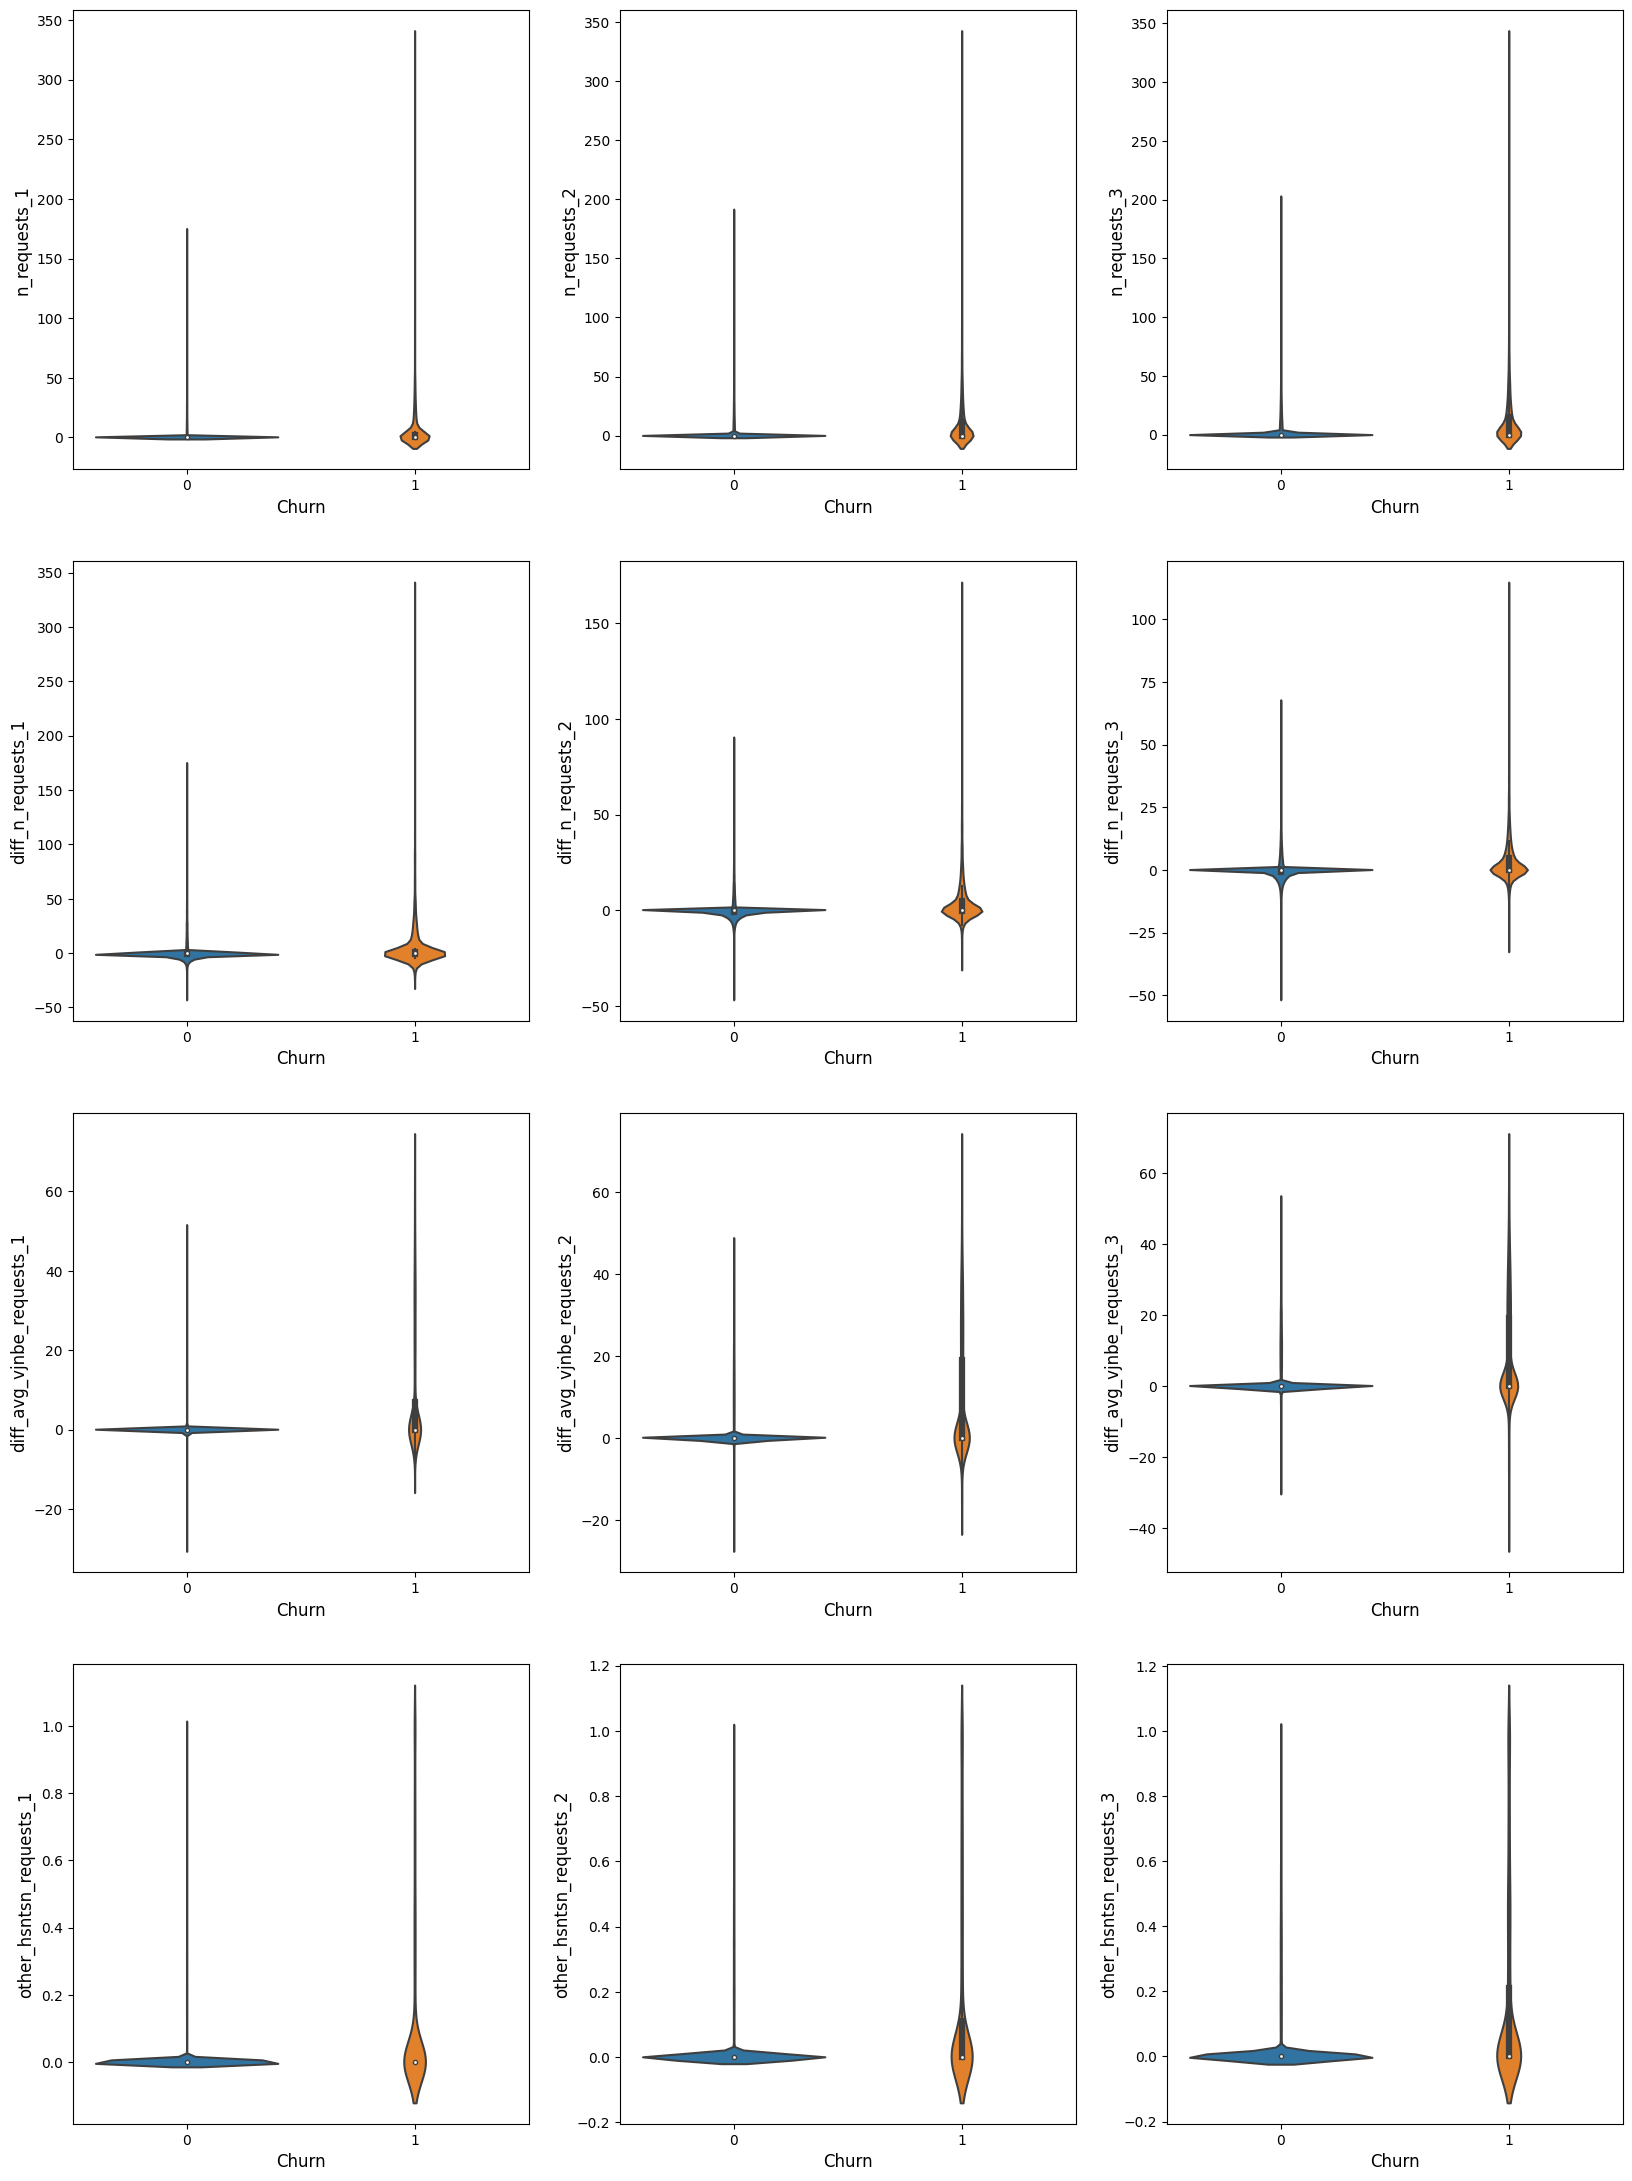
\includegraphics[height=23cm]{violin1.png}}
\caption{Violinplots for Quotation Variables}
\label{fig:edaq}
\end{figure}
\begin{figure}[H]
    \centerline{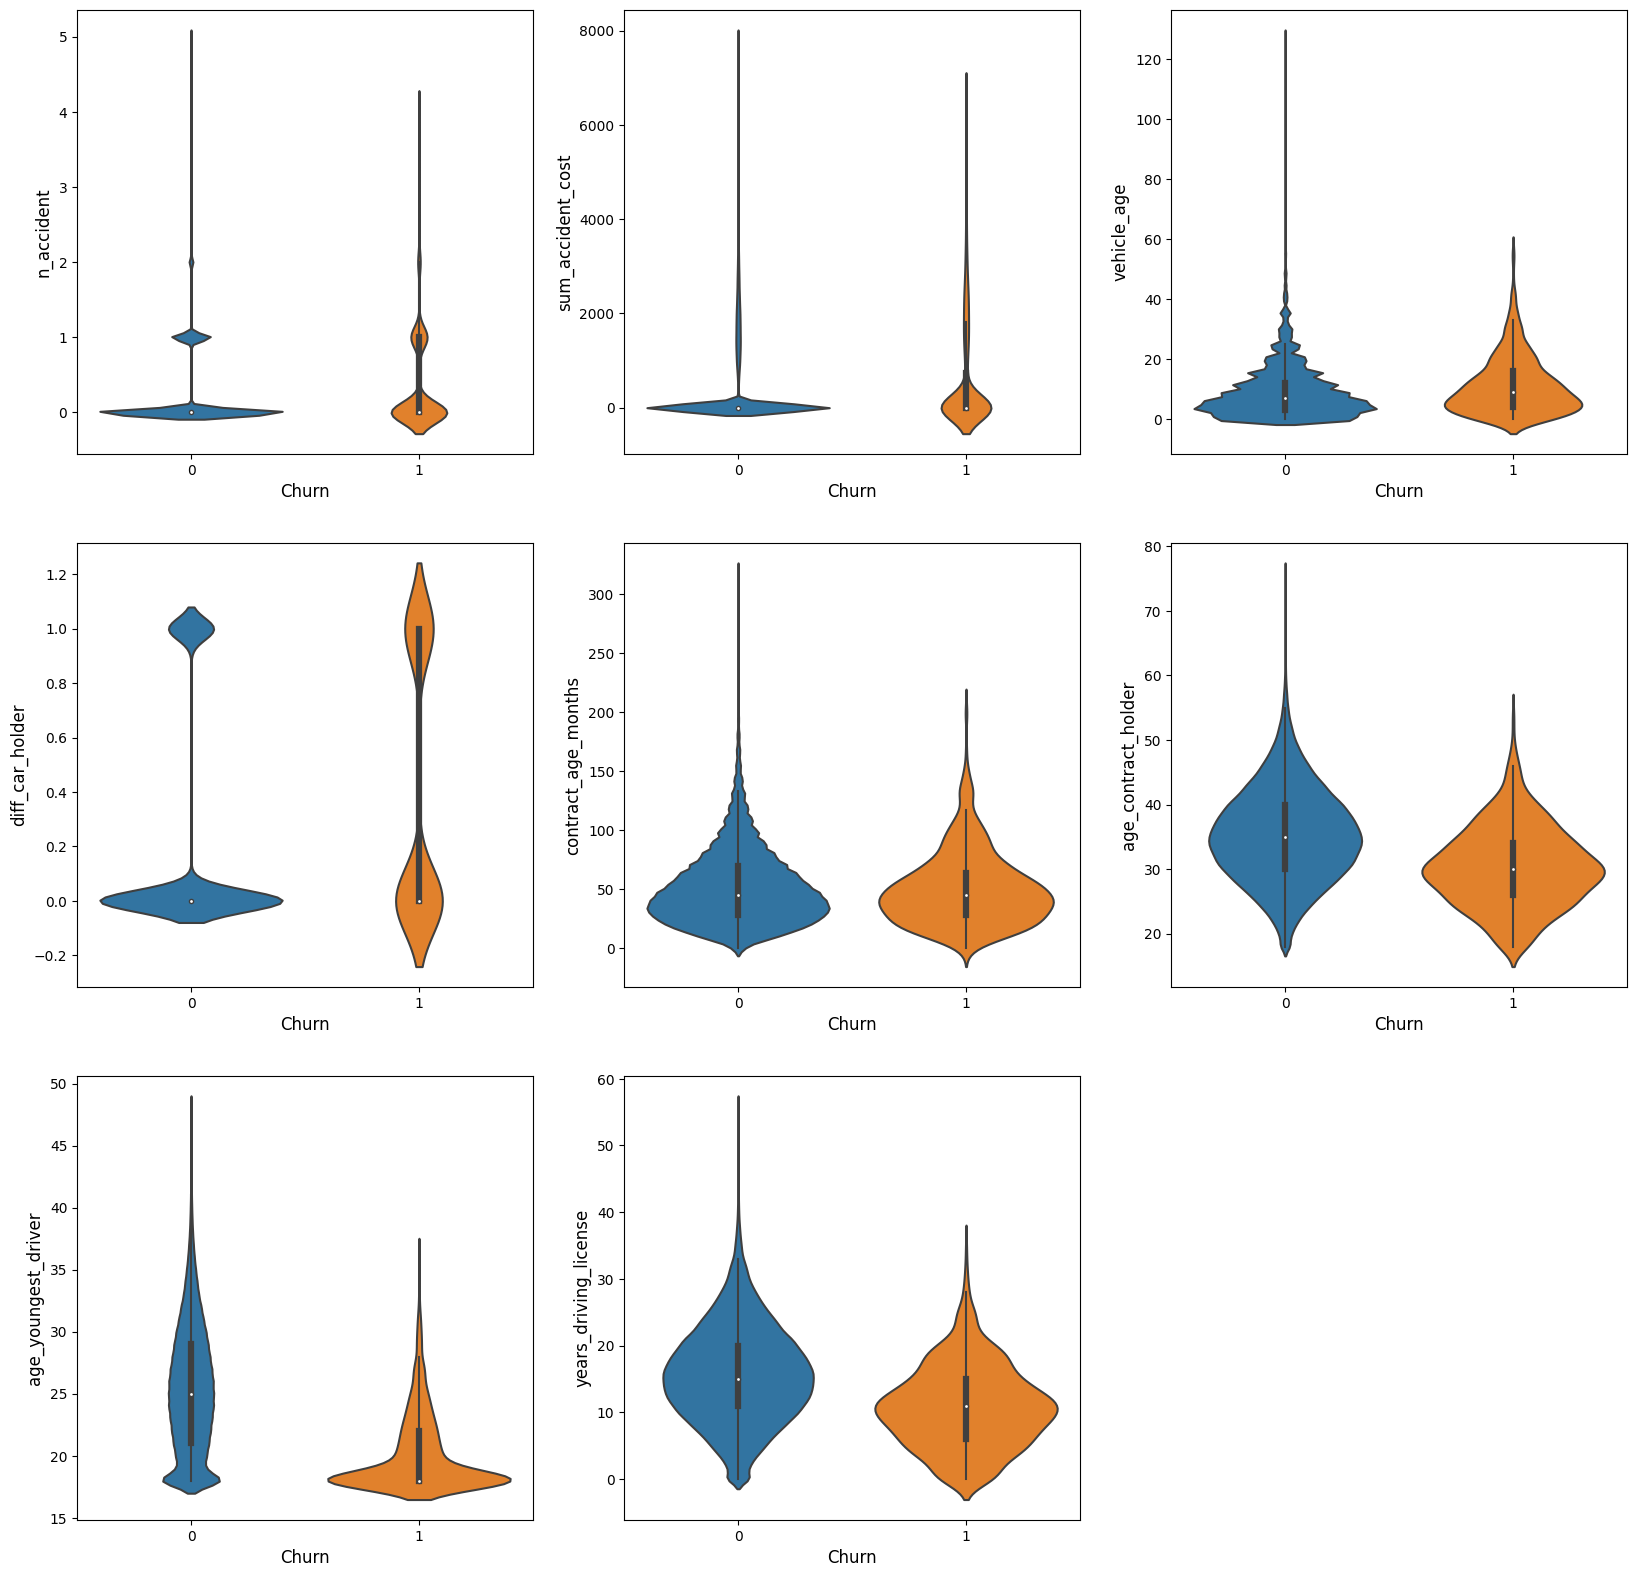
\includegraphics[height=17cm]{violin2.png}}
\caption{Violinplots for Non-Quotation Variables}
\label{fig:edanq}
\end{figure}

\noindent
The key insights that are generated through exploring the data point at the effectiveness and importance of including quotation data in churn modelling. (1) There are significant differences in the averages and the standard deviations (the distribution in general) in the number of requests generated 1, 2 and 3 months before $t$, when comparing the group of churners with the group of non-churners. The relative difference is the highest for "n\_requests\_1", with an average of $0.96$ for non-churners versus $6.26$ for churners, and a standard deviation of $6.15$ versus $18.32$. \\
Note that the distribution is heavily right skewed, which is represented by the median being $0$ for both groups. This indicates that the majority of customers, for both customers with and without a willingness to churn, do not generate requests. \\
Other key insights include but are not limited to the following: (2) The average (and standard deviation) of "diff\_n\_requests\_1" with $4.95$ (and $18.54$) for churners is also significantly larger than $0.01$ (and $6.45$) for non-churners. This reflects that the request behavior of customers which are about to churn changes significantly, while non-churners show the same behavior. \\
(3) The average calculated price for churners was significantly higher than the price they are paying in their contract. This is reflected in the means of "diff\_avg\_vjnbe\_requests\_1" with a difference of $15.00$. For non-churners this difference is also positive but only around $20\%$ as high. \\
(4) A proportion of churners do search for different cars than their current car in their request. This is reflected by the average of "other\_hsntsn\_requests\_1" for churners being $0.10$. This average is smaller for non-churners with $0.01$. \\
(5) Regaring non-quotation variables, most noticeable are the significantly lower averages and medians for churners in terms of the age variables, espacially "age\_youngest\_driver". \\

\subsection{Modelling Baseline} \par

To get an idea on how well a specific model is performing it is useful to have a baseline for the evaluation metrics. Typically the baseline is a simple model/solution. When applying a new solution to solve a business problem, stakeholders are predominantly interested in the generated improvement in terms of profit (or other business KPIs). Thereofore in this context, the status quo is selected as the baseline in most cases. Wether the solution achieves an improvement over the status quo is decisive for the implementation of it. \\
In the application of this work, the status quo consists of the no-existence of any mid-contract-period churn prediction model. The fact that quotation data availability and quality was ensured only a few months before this work is the reason for it. As this work underlines the importance and predictive power of quotation data in churn contexts, earlier attempts of modelling this problem were unsuccessful. \\
Hence, the most naïve baseline we can set for our modelling is that mid-contract-period churns are never predicted. We name and index this baseline with "B1". Applying this rule to compute the confusion matrix both on the out-of-sample (OOS) and out-of-period (OOP) test data, we are left with following results: \\
\noindent
\begin{figure}[H]
\centering
\begin{subfigure}{.5\textwidth}
  \centering
  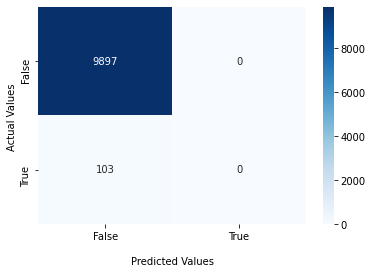
\includegraphics[width=1\linewidth]{conf_b1_oos.png}
  \caption{OOS}
  \label{fig:conf_b1_oos}
\end{subfigure}%
\begin{subfigure}{.5\textwidth}
  \centering
  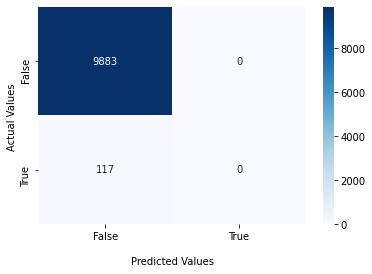
\includegraphics[width=1\linewidth]{conf_b1_oop.png}
  \caption{OOP}
  \label{fig:conf_b1_oop}
\end{subfigure}
\caption{Baseline 1 (B1); Status Quo}
\label{fig:b1}
\end{figure}
\vspace{5mm}
We introduce another baseline which is based on a simple decision rule. This decision rule leads to a prediction of churn if the specific customer showed quotation activity in the past month. This implies: \\
\vspace{5mm}
\noindent
\begin{equ}[H]
\begin{equation} \label{b2}
    \widehat{C_{t+s}^{class}} = \begin{cases}
        1,& \text{if } n\_requests_{t - 1, t} > 1 \\
        0,& \text{if } n\_requests_{t - 1, t} = 0
    \end{cases}
\end{equation}
\end{equ}
\vspace{1mm}

\noindent
The resulting confusion matrices for OOS and OOP from this baseline (B2) are plotted in figure \ref{fig:b2}. \\
\noindent
\begin{figure}[H]
\centering
\begin{subfigure}{.5\textwidth}
  \centering
  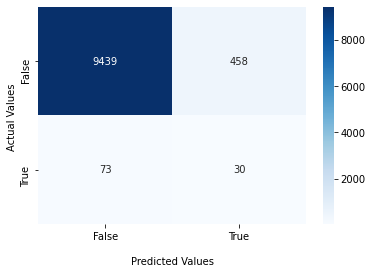
\includegraphics[width=1\linewidth]{conf_b2_oos.png}
  \caption{OOS}
  \label{fig:conf_b2_oos}
\end{subfigure}%
\begin{subfigure}{.5\textwidth}
  \centering
  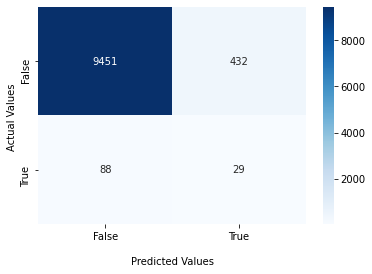
\includegraphics[width=1\linewidth]{conf_b2_oop.png}
  \caption{OOP}
  \label{fig:conf_b2_oop}
\end{subfigure}
\caption{Baseline 2 (B2); Quotation Activity}
\label{fig:b2}
\end{figure}
\vspace{5mm}
We further summarize all evaluation matrices for B1 and B2 we are interested in and we want improve on with our modelling approach in table \ref{tab:baseline}. \\
\noindent
\setlength{\tabcolsep}{5pt}
\renewcommand{\arraystretch}{1.2}
\begin{table}[H]
    \centering
    \begin{tabular}{|l|cccccc|}
    \hline
              & Accuracy & Precision & Recall &   F1   & AUROC & AUPRC  \\
    \hline
    B1 on OOS &  0.9897  &   0.0000  & 0.0000 & 0.0000 & 0.5000 & 0.0103 \\
    B1 on OOP &  0.9883  &   0.0000  & 0.0000 & 0.0000 & 0.5000 & 0.0117 \\
    \hline
    B2 on OOS &  0.9469  &   0.0615  & 0.2913 & 0.1052 & 0.6225 & 0.0252 \\
    B2 on OOP &  0.9480  &   0.0629  & 0.2479 & 0.1003 & 0.6021 & 0.0244 \\
    \hline
    \end{tabular}
    \caption{Baseline Evaluations on Test Data}
    \label{tab:baseline}
\end{table}

\subsection{Modelling Results} \par

While presenting the results we want to emphasize, that for both modelling approaches GBT and EBM we use figure \ref{fig:shptl} representing one iteration of the Structural-HP-Tuning-Loop (S-HPTL) as the modelling structure. The Model-HP-Tuning-Loop (M-HPTL) and the Structural-HP-Tuning-Loop (S-HPTL) are in depth explained in chapter \ref{chap:modstruct}. During M-HPTL, for each hyperparameter we sample from the corresponding set presented in table X for GBT and from table Y for EBM. \\
We of course do not present each of the fits performed in the inner loop (M-HPTL). Remember, that the M-HPTL nests in each iteration of the S-HPTL, which further increases the number of total fits. Therefore, we focus only on the M-HPTL optimal result, which is essentially one best model-hyperparameter set, its trained model and its evaluation scores. \\

\subsubsection*{(i) Gradient Boosted Trees Results}

Before presenting the results we want to make some additional notational remarks. We denote the best model resulting from M-HPTL for a specific iteration of S-HPTL by: "gbt\_\{sampling method\}\_\{custom loss parameters\}". So for example "gbt\_d0.1\_a0.6g2" represents the best model with a downsampled dataset with factor $0.1$ and with a focal loss implementation of $\alpha=0.6$ and $\gamma=2$. Also, for now we concentrate on the models fitted including the best set of quotation variables. This is why this notation does not include an indicator for which variables are used. With the best model at hand however we compare both with and without quotation variables results in order to show the importance of them. \\
Moreover we do not present the resulting best model from each S-HPTL iteration, as we have $8\times4\times6\times2=384$ iterations in total. We focus on the main insights and present the best results in terms of evaluation metrics in table \ref{tab:gbteval}. \\
\setlength{\tabcolsep}{3pt}
\renewcommand{\arraystretch}{1.5}
\begin{table}[h!]
    \centering
    \noindent
    \begin{tabular}{|lc|cccccc|}
    \hline
    Model                              & Test-Set & Accuracy        & Precision       & Recall          & F1              & AUROC           & AUPRC            \\ 
    \hline
    \multirow{2}{*}{\textbf{gbt\_u10\_aNgN}}    & OOS      & \textbf{0.9857} & \textbf{0.3246} & 0.3592          & \textbf{0.3410} & 0.8782          & 0.3231           \\ 
    \cdashline{2-8}[1pt/1pt]
                                       & OOP      & \textbf{0.9843} & \textbf{0.2727} & 0.2051          & 0.2341          & 0.8438          & 0.1909           \\ 
    \hline
    \multirow{2}{*}{gbt\_d0.1\_aNgN}   & OOS      & 0.9790          & 0.2390          & 0.4757          & 0.3182          & 0.8921          & 0.3267           \\ 
    \cdashline{2-8}[1pt/1pt]
                                       & OOP      & 0.9767          & 0.1947          & 0.3162          & \textbf{0.2410} & 0.8485          & \textbf{0.2070}  \\ 
    \hline
    \multirow{2}{*}{gbt\_u\_aNgN}      & OOS      & 0.9162          & 0.0761          & 0.6408          & 0.1361          & 0.8791          & 0.3310           \\ 
    \cdashline{2-8}[1pt/1pt]
                                       & OOP      & 0.9126          & 0.0733          & 0.5556          & 0.1295          & 0.8389          & 0.1956           \\ 
    \hline
    \multirow{2}{*}{gbt\_d0.1\_a0.6gN} & OOS      & 0.9702          & 0.1803          & 0.5340          & 0.2696          & \textbf{0.9032} & \textbf{0.3338}  \\ 
    \cdashline{2-8}[1pt/1pt]
                                       & OOP      & 0.9645          & 0.1234          & 0.3333          & 0.1801          & \textbf{0.8577} & 0.1924           \\ 
    \hline
    \multirow{2}{*}{gbt\_u\_a0.8gN}    & OOS      & 0.8487          & 0.0487          & 0.7379          & 0.0913          & 0.8746          & 0.2972           \\ 
    \cdashline{2-8}[1pt/1pt]
                                       & OOP      & 0.8378          & 0.0442          & 0.6239          & 0.0826          & 0.8251          & 0.1923           \\ 
    \hline
    \multirow{2}{*}{gbt\_u50\_aNg0.5}  & OOS      & 0.8970          & 0.0530          & 0.5340          & 0.0965          & 0.8452          & 0.0498           \\ 
    \cdashline{2-8}[1pt/1pt]
                                       & OOP      & 0.8884          & 0.0463          & 0.4360          & 0.0837          & 0.8045          & 0.0385           \\ 
    \hline
    \multirow{2}{*}{gbt\_sm\_aNg2}     & OOS      & 0.8285          & 0.0462          & 0.7961          & 0.0873          & 0.8808          & 0.1267           \\ 
    \cdashline{2-8}[1pt/1pt]
                                       & OOP      & 0.8157          & 0.0405          & 0.6496          & 0.0762          & 0.8293          & 0.0732           \\ 
    \hline
    \multirow{2}{*}{gbt\_u50\_a0.6g1}  & OOS      & 0.8973          & 0.0471          & 0.4660          & 0.0855          & 0.7909          & 0.0340           \\ 
    \cdashline{2-8}[1pt/1pt]
                                       & OOP      & 0.8872          & 0.0433          & 0.4102          & 0.0784          & 0.7786          & 0.0324           \\ 
    \hline
    \multirow{2}{*}{gbt\_sm\_a0.7g2}   & OOS      & 0.5378          & 0.0196          & \textbf{0.8932} & 0.0383          & 0.8074          & 0.0397           \\ 
    \cdashline{2-8}[1pt/1pt]
                                       & OOP      & 0.5237          & 0.0208          & \textbf{0.8632} & 0.0406          & 0.7864          & 0.0358           \\
    \hline
    \end{tabular}
    \caption{Evaluation of GBT-Candidates on Test Data}
    \label{tab:gbteval}
\end{table}

First insights which are generated through looking at the results are the following: \\
(1) The out-of-period evaluation scores for almost all models are lower than the ones for out-of-sample. This holds true for almost all applications and was expected. As churn rates differ from period to period, we intentionally raised the amount of churners by 10\% to also evaluate robustness over time of the model candidates. \\
(2) Sampling towards a balanced training data set in general creates confidence in the model to predict the minority class. This is reflected in a dropping precision and a rising recall. \\
(3) Eventhough SMOTE is said to be a more advanced and reliable approach than upsampling, the latter yields better results in our application.\\
(4) Using weights $\alpha$ in the loss functions delivers same results to sampling in terms of confidence. Additionally with a too high $\alpha$ (starting at $\alpha=0.7$) the F1-Score and the AUPRC start to drop.\\
(5) Adding $\gamma\neq0$ to the loss, we also observe confidence in the model, but this confidence is not restricted towards predicting the minority class. Paired with a low $\alpha$ a too high $\gamma$ ($>1$) can have backfiring effects and lead to no predictions of the minority class. When a too high $\gamma$ is paired with a high $\alpha$ however, the model fit can lead to only predicting the minority class. The main takeaway for the usage of focal loss is to carefully select the parameters, as with wrong calibration it can lead to overconfidence. \\
(6) Eventhough using a cost-sensitive loss function is highly suggested in the literature, standard sampling methods alone or paired with a cost-sensitive loss yield better and more robust results in our application. \\

\subsubsection*{Best GBT model candidate}

Due to the high class imballance, the main evaluation metrics we look at in this work are the AUPRC and the F1-Score. There is no candidate which scores highest in both metrics. Nevertheless "gbt\_u10\_aNgN" has by far the highest F1-Score and only lacks a small amount behind other candidates in terms of AUPRC. Therefore the model that represents our best GBT candidate is obtained with an upsampled ($\times 10$) minority class and no cost-sensitive loss function. "n\_requests\_1", "diff\_n\_requests\_3", "diff\_avg\_vjnbe\_requests\_3" and "other\_hsntsn\_requests\_3" are used as the optimal quotation variable set resulting from MRMR dimension reduction. \\
The trained model yields a 224\% (and 133\%) improvement in the F1-Score on OOS (and OOP) data over the Baseline 2. The increase in AUPRC on OOS (and OOP) data for B2 amounts to 1182\% (and 682\%). \\
"gbt\_u10\_aNgN"'s evaluation scores are much higher with the best set of quotation variables than without, which highlights its predictive power. The absolute deviation of the F1-Score without quotation variables on OOS data lies at $-0.2234$, for OOP at $-0.1267$. The AUPRC is $0.2515$ lower for OOS data and for OOP $0.1342$ lower. This fact also holds true for all other GBT candidates. Table \ref{gbtevalimprov} in the appendix summarizes the gain in the evaluation metrics generated through the inclusion of quotation data for all candidates. \\

\subsubsection*{Interpretation of GBT candidate}

We use "gbt\_u10\_aNgN" to shed light on this black-box in order to make it interpretable. Therefore we make use of explainability methods PDP and SHAP. Both methods are explained in chapter \ref{section:interpreting}. \\
\noindent
\begin{figure}[h!]
\centering
    \begin{subfigure}{.55\textwidth}
      \centering
      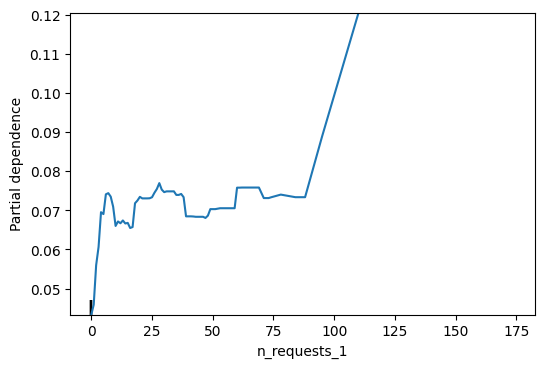
\includegraphics[width=1\linewidth]{pdp_n_requests_1.png}
    \end{subfigure}%
    \begin{subfigure}{.55\textwidth}
      \centering
      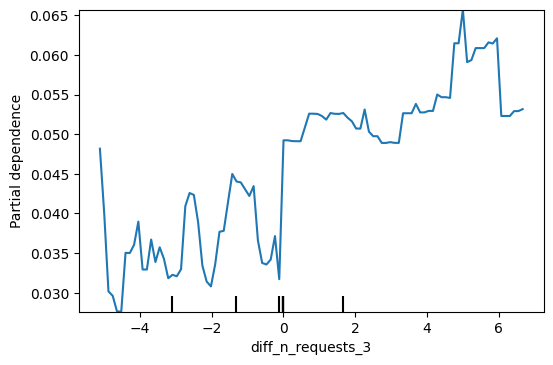
\includegraphics[width=1\linewidth]{pdp_diff_n_requests_3.png}
    \end{subfigure} \\
    \begin{subfigure}{.55\textwidth}
        \centering
        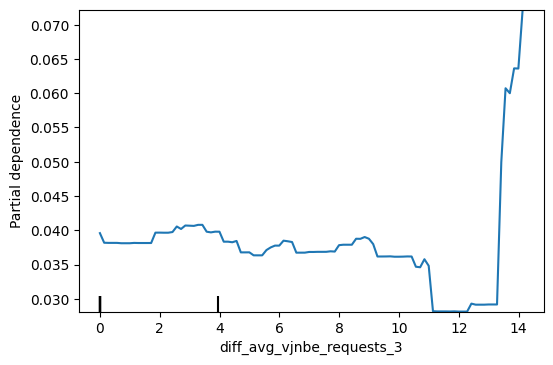
\includegraphics[width=1\linewidth]{pdp_diff_avg_vjnbe_requests_3.png}
    \end{subfigure}%
    \begin{subfigure}{.55\textwidth}
        \centering
        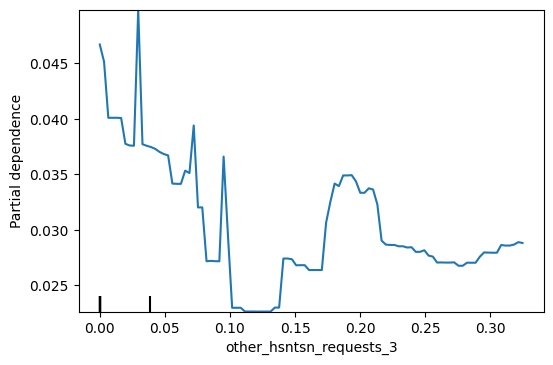
\includegraphics[width=1\linewidth]{pdp_other_hsntsn_requests_3.png}
    \end{subfigure} \\
    \begin{subfigure}{.55\textwidth}
        \centering
        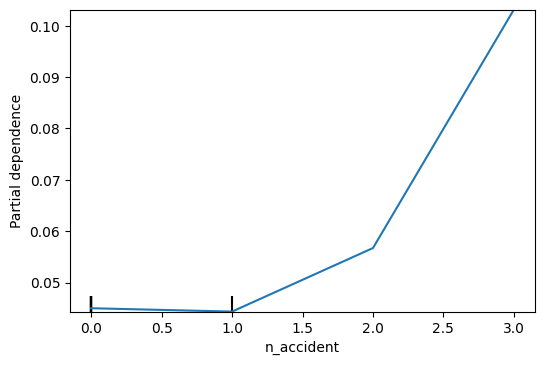
\includegraphics[width=1\linewidth]{pdp_n_accident.png}
    \end{subfigure}%
    \begin{subfigure}{.55\textwidth}
        \centering
        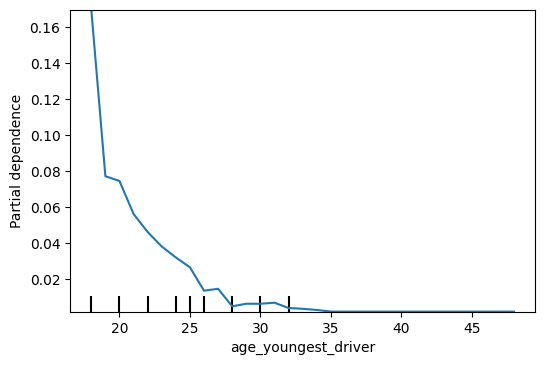
\includegraphics[width=1\linewidth]{pdp_age_youngest_driver.png}
    \end{subfigure} \\
\caption{Partial dependency plots (PDP) for GBT}
\label{fig:pdp}
\end{figure}

Figure \ref{fig:pdp} presents the PDP's for the main drivers behind this model. The first graph represents the PDP for variable "n\_requests\_1" and confirms the hypothesis of a strong positive relationship between it and the probability of a churn. The relationship shown for "diff\_n\_requests\_3" is also as expected, the higher the difference of quotation activity to the normal behavior the higher the probability of a churn. The insights generated through the PDP's for the remaining two quotation variables do not show the expected relationship. This however can be caused by the disadvantage of PDP's when facing correlated explanatory variables. \\
The lower two graphs show the two non-quotation variables which have the strongest relationship with the target variable. On the left we see that the number of accidents since the start of the contract go along with a higher predicted probability on average. Considering the fact, that an accident gives customers the exceptional right of mid-contract-period termination, this relationship is intuitive. More importantly, following an accident the insurer raises the insurance fee in most cases which obviously raises the probability of a churn. \\
The strongest partial dependency relationship is shown in the age of the youngest driver registered in the contract. The explanation for this effect may be that driving-license-freshers are typically first registered in the insurance contract of their parents or other relatives. As a reaction insurance companies raise the insurance fee, as young drivers typically pose a higher risk for accidents. The reaction of the customer is a higher probability of churn. \\

Figure \ref{fig:shapsum} visualizes SHAP's summary-plot, a method  to transform the local model-agnostic method of SHAP to a globally interpretable one. Each dot represents one sample and the contribution of its corresponding variable value (y-axis) to the predicted log-odds (x-axis). The insights of this plot are almost all inline with the ones from PDP. Most dominant are the average contributions of "age\_youngest\_driver" to the log odds. It also hints at a negative relationship, the one with highest impact on the predictions, which is inline with PDP. \\
In this summary plot, SHAP shows new insights on the model behavior for "diff\_avg\_vjnbe\_requests\_3". More precisely, for some samples a high deviation between the average price shown during the requests and the contract fee increases the predicted probability by the most among all variable contributions. \\
\begin{figure}[H]
    \centerline{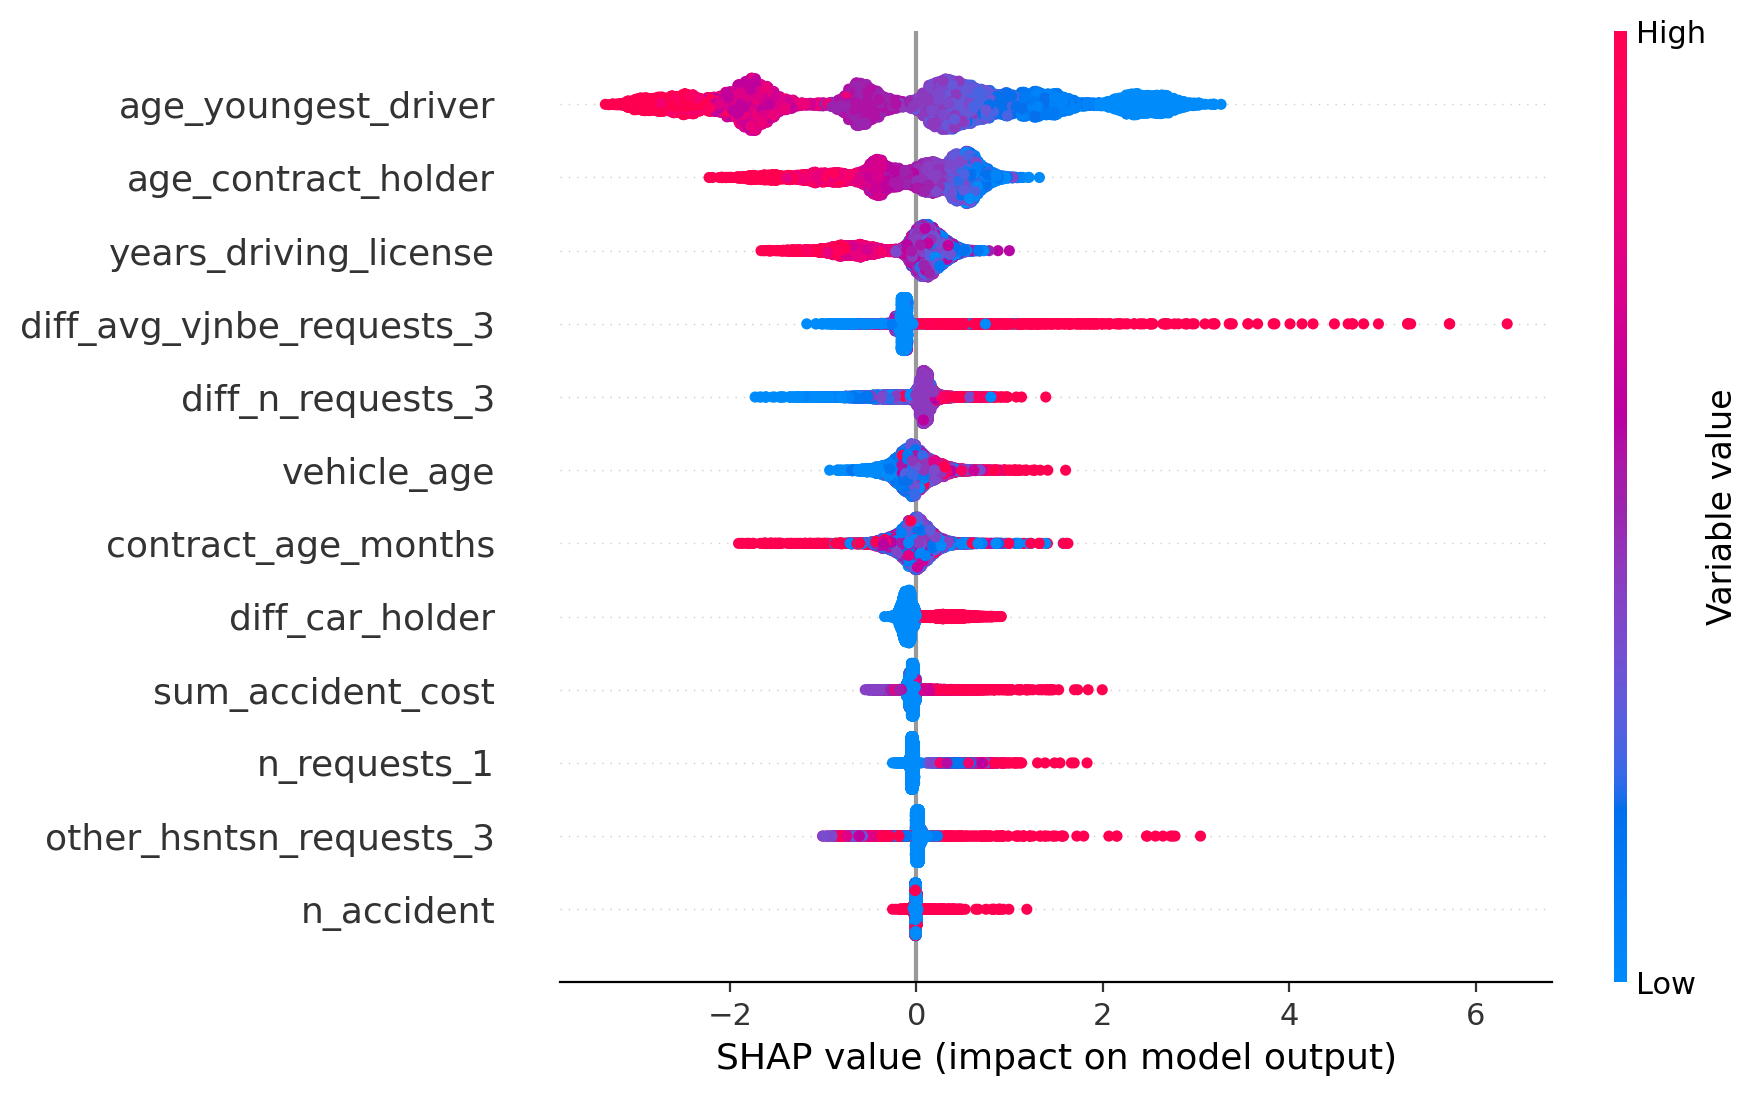
\includegraphics[height=10cm]{shap_summary.png}}
\caption{SHAPs Summary Plot on GBT candidate Model}
\label{fig:shapsum}
\end{figure}
\noindent
The SHAP-values of a single prediction also provide a good explanations of how the prediction is generated and how each variable value contributed. In our context of customer churn single explanations can be applied on predicted churners before taking any action (call customer or give rebates) to fully understand the reason of the prediction. Figure \ref{fig:shapsum} shows how the SHAP-Values can be visualized. There, each bar visualizes the estimated Shapley value $\delta^{(j)}$ of the corresponding variable value. Stacking all bars on top of each other results in a representation on how the predicted log differs from the sample mean.\\
\begin{figure}[H]
    \centerline{
\includegraphics[height=8cm]{shap_waterfall_example.png}}
    \caption{SHAPs Summary Plot on GBT candidate Model}
    \label{fig:shapsum}
\end{figure}
\noindent
In this example, the difference in the average price shown during the requests has the highest contribution to the prediction. This customer also has a young driver registered which also rises the model probability. The fact, that 95\% of the requests belonging to that customer included a different car than the one in his contract, has the third highest contribution. All other variable values only have minor contributions for this example. \\
This concludes the result presentation of the GBT modelling approach. We present 9 candidate models, all using different sets of sampling methods, loss functions and explanatory variables. The best model turns out to be the result of an upsampling approach in combination with no cost-sensitive loss-function. The quotation data shows to have high predictive power for GBT and we used explainability methods to examine the relationship between prediction and the main drivers of the model. In the next section we compare these results with the EBM approach. \\

\subsubsection*{(ii) Explainable Boosting Machine Results}

Also, regarding the best model resulting from M-HPTL for a specific iteration of S-HPTL we use a similar notation: "ebm\_\{sampling method\}". We again first only present model performances of EBM candidates including the best set of quotation variables. With the best model at hand however we compare both with and without quotation data results in order to show the relevance of quotation data. Table \ref{tab:ebmeval} summarizes the best 5 models and their OOS and OOP performances.\\

\begin{table}[h!]
    \centering
    \begin{tabular}{|lc|cccccc|}
    \hline
    Model                              & Test-Set & Accuracy        & Precision       & Recall          & F1              & AUROC           & AUPRC            \\ 
    \hline
    \multirow{2}{*}{ebm\_none}    & OOS      & \textbf{0.9912} & \textbf{0.8000} & 0.1942          & 0.3125 & 0.5968          & 0.1636           \\ 
    \cdashline{2-8}[1pt/1pt]
                                       & OOP      & \textbf{0.9892} & \textbf{0.7647} & 0.1111          & 0.1940          & 0.5554          & \textbf{0.0954}           \\
    \hline
    \multirow{2}{*}{ebm\_d0.1}   & OOS      & 0.9821          & 0.2683          & 0.4272          & 0.3296          & 0.7075          & 0.1205           \\ 
    \cdashline{2-8}[1pt/1pt]
                                       & OOP      & 0.9808          & 0.2302          & 0.2735          & \textbf{0.2500} & 0.6313          & 0.0715  \\ 
    \hline
    \multirow{2}{*}{\textbf{ebm\_d0.5}}      & OOS      & 0.9911          & 0.6750          & 0.2621          & \textbf{0.3776}          & 0.6304          & \textbf{0.1845}           \\ 
    \cdashline{2-8}[1pt/1pt]
                                       & OOP      & 0.9885          & 0.5294          & 0.1538          & 0.2384          & 0.5761          & 0.0913           \\ 
    \hline
    \multirow{2}{*}{ebm\_d} & OOS      & 0.8050          & 0.0412          & \textbf{0.8058}          & 0.0784          & \textbf{0.8054} & 0.0352  \\ 
    \cdashline{2-8}[1pt/1pt]
                                       & OOP      & 0.7941          & 0.0420          & \textbf{0.7607}          & 0.0796          & \textbf{0.7776} & 0.0347           \\ 
    \hline
    \multirow{2}{*}{ebm\_u10}    & OOS      & 0.9822          & 0.2582          & 0.3883          & 0.3101          & 0.6884          & 0.1065           \\ 
    \cdashline{2-8}[1pt/1pt]
                                       & OOP      & 0.9805          & 0.2090          & 0.2393          & 0.2231          & 0.6143          & 0.0589           \\ 
    \hline
    \end{tabular}
    \caption{Evaluation of EBM-Candidates on Test Data}
    \label{tab:ebmeval}
\end{table}
\noindent
This table delivers following insights regarding best sampling methods and comparison to GBT: \\
(1) The F1-Score is comparable to - and for one candidate even higher than - the GBT candidates. The AUROC and AUPRC however are lower for all EBM-candidates. \\
(2) For almost all EBM-candidates, the differences between OOS and OOP evaluation scores are as high as for GBT. \\
(3) Same observations apply for EBM as for GBT in terms of sampling effectiveness and implications on evaluation metrics. \\

\subsubsection*{Best EBM model candidate}

Looking at the AUPRC and the F1-Score, "ebm\_d0.5" scores the best on the OOS set. Eventhough it is not the best candidate in terms of OOP evaluation, there is no other candidate which outperforms it in both metrics on OOP data. Therefore we pick this model using a downsampled ($\times 0.5$) training data set as the best EBM-candidate. The quotation variables which survived the MRMR-filtering are also: "n\_requests\_1", "diff\_n\_requests\_3", "diff\_avg\_vjnbe\_requests\_3" and "other\_hsntsn\_requests\_3". Optimal interactions which are detected with the FAST algorithm are: \\

\vspace{3mm}
\textit{(1)} diff\_avg\_vjnbe\_requests\_3 x age\_youngest\_driver \par
\textit{(2)} diff\_avg\_vjnbe\_requests\_3 x n\_accident \par
\textit{(3)} other\_hsntsn\_requests\_3 x vehicle\_age \par
\textit{(4)} diff\_avg\_vjnbe\_requests\_3 x age\_contract\_holder \par
\textit{(5)} diff\_avg\_vjnbe\_requests\_3 x years\_driving\_license \par
\textit{(6)} diff\_avg\_vjnbe\_requests\_3 x contract\_age\_months \par
\textit{(7)} diff\_avg\_vjnbe\_requests\_3 x other\_hsntsn\_requests\_3 \par
\textit{(8)} diff\_avg\_vjnbe\_requests\_3 x sum\_accident\_cost \par
\textit{(9)} n\_requests\_1 x age\_youngest\_driver \\
\vspace{1mm}

\noindent
The trained EBM-model yields a 258\% (and 126\%) improvement in the F1-Score OOS (and OOP) over the Baseline 2. The increase in AUPRC OOS (and OOP) for B2 amounts to 632\% (and 262\%). \\
The EBM modelling approach also highlights the predictive power of quotation data in churn prediction application. Absolute differences in the F1-Score without quotation variables constitute to $-0.3776$ for OOS evaluation, for OOP to $-0.2216$. The AUPRC is $0.1742$ lower for OOS data, for OOP $0.0754$ lower. This effect is also visable for all other candidates of EBM and is summarized in table \ref{ebmevalimprov} in the appendix. \\

\subsubsection*{Interpretation of EBM candidate}

EBM's big advantage is its simple interpretability. The addition of the individual values from the shape functions forms the log odds. Each shape function takes at most 2 explanatory variables (2 for interactions) as input. Therefore plotting these shape functions tells us the relationship of variable (or variable interaction) and predicted log odds. Also, because of the additive model structure, local and global interpretations are equal for EBM. \\
\begin{figure}[H]
    \centering
        \begin{subfigure}{.55\textwidth}
          \centering
          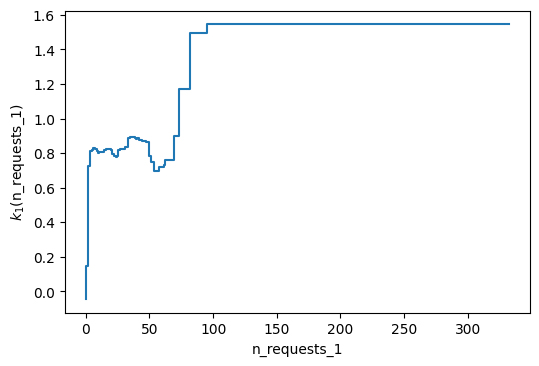
\includegraphics[width=1\linewidth]{shape_function_n_requests_1.png}
        \end{subfigure}%
        \begin{subfigure}{.55\textwidth}
          \centering
          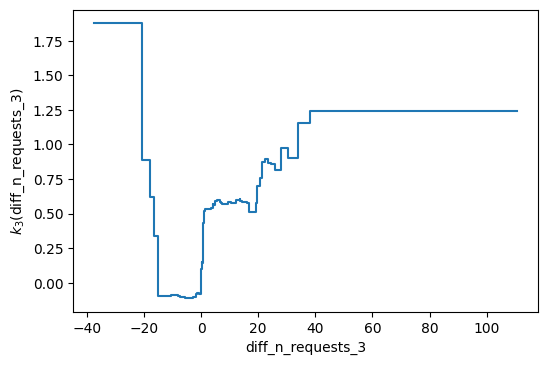
\includegraphics[width=1\linewidth]{shape_function_diff_n_requests_3.png}
        \end{subfigure} \\
        \begin{subfigure}{.55\textwidth}
            \centering
            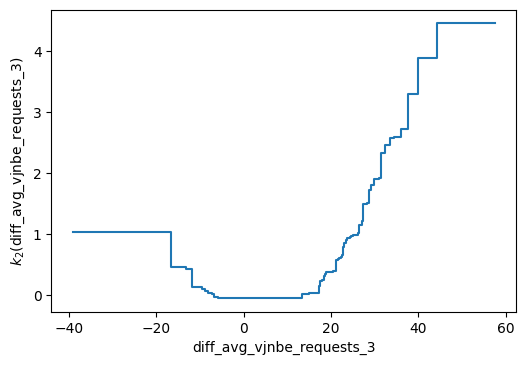
\includegraphics[width=1\linewidth]{shape_function_diff_avg_vjnbe_requests_3.png}
        \end{subfigure}%
        \begin{subfigure}{.55\textwidth}
            \centering
            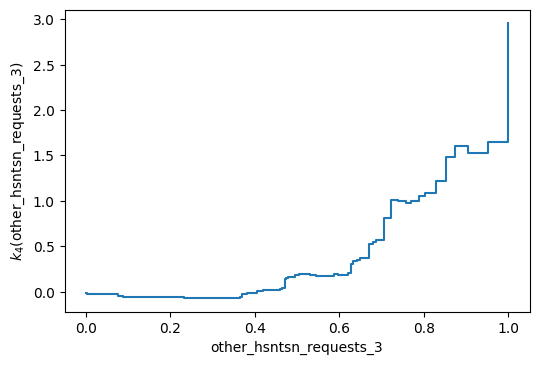
\includegraphics[width=1\linewidth]{shape_function_other_hsntsn_requests_3.png}
        \end{subfigure} \\
        \begin{subfigure}{.55\textwidth}
            \centering
            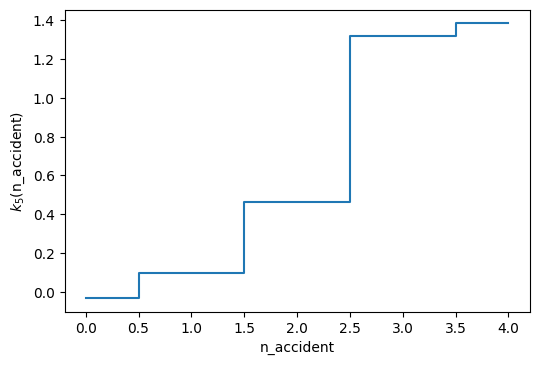
\includegraphics[width=1\linewidth]{shape_function_n_accident.png}
        \end{subfigure}%
        \begin{subfigure}{.55\textwidth}
            \centering
            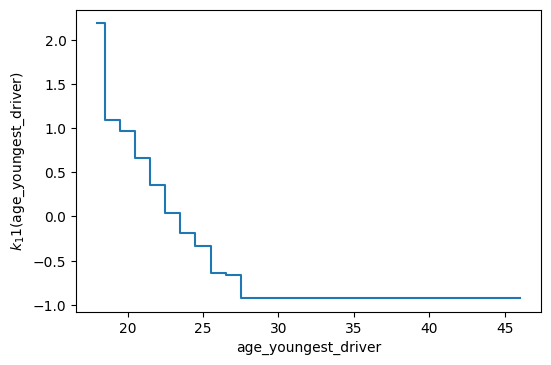
\includegraphics[width=1\linewidth]{shape_function_age_youngest_driver.png}
        \end{subfigure} \\
    \caption{Shape functions of EBM}
    \label{fig:shapefct}
\end{figure}
\noindent
Figure \ref{fig:shapefct} shows the main drivers for the best performing EBM candidate. Note that the plots should be interpreted carefully and should not be falsely compared to the PDP plots. Note, that in contrast to the PDPs for GBT, the y-axis now represents the value of the shape function. For a specific variable value, the value of the shape function is its additive contribution to the log odds. \\
What stands out in this figure is that quotation variables have stronger relationships with the log odds (and therefore also with the predicted probability of a churn) than non-quotation variables. This insight again strongly supports the inclusion of quotation variables for churn modelling. \\
Additionally, all plots show the expected behavior of variable-target relationships. For "n\_requests\_1" for example, the log-odds contribution rises sharply from below 0 to 0.8 for more than 0 requests. Except the drop at around 55 requests, the contribution rises steadily to 1.5 for more than 100 requests. \\
The plot for "diff\_n\_requests\_3" shows the expected behavior for positive deviations, but also generates a new hypothesis for negative deviations. The peculiarity is the again sharply rising contribution at around diff\_n\_requests\_3 $=-17$. It could be explained by the phenomenon, that customers who normally have high quotation activity but did not show them in the last 3 months have already predecided to only look for other insurers before churning. This relationship was not visable with explainability approaches for GBT. \\
The strongest contributions to the log odds are generated by rising deviations in request-price versus contract-price and an increasing percentage of deviating car searches. For "diff\_avg\_vjnbe\_requests\_3" $=40$ the contribution reaches a value of 4, whereas with 100\% deviating car searches the contribution amounts to around 2.9. \\
The best non-quotation variables also show an expected relationship. "n\_accident"'s contribution to the log odds rises approximately linearly from 0 to 1.4 for 4 accidents in the contract period. A negative relationship is shown by the age of the youngest driver and its contribution, until the age reaches 28. For older youngest drivers it stays stable at around -0.9. \\
Eventhough the interaction variables do not show strong contributions on the log odds, we present one example interaction of "diff\_avg\_vjnbe\_requests\_3" and "n\_accident" in Figure \ref{fig:shape2dim}. It is an example for how even interactions can be visualized and interpreted. All other variables and variable pairs only have a comparably weak relationship and are therefore not presented. \\
\begin{figure}[H]
    \centerline{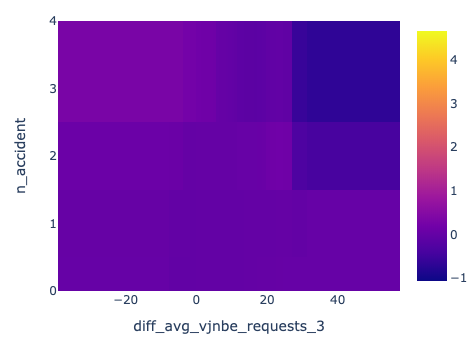
\includegraphics[height=7cm]{shape_2dim.png}}
    \caption{Relationship of Interaction Term and Log Odds}
    \label{fig:shape2dim}
\end{figure}
\noindent
To summarize the results for the EBM approach we present 5 candidate models, all using different sets of sampling methods and explanatory variables. Downsampling the majority class by 50\% and including the best set of quotation variables yields the best evaluation scores. Plots of individual shape functions enable to easily examine relationships between log odds and variable of interest. Besides confirming preassumptions made for relationships, the plot give new insights. We are now able to compare both modelling approaches and simulate their improvement over the status quo, when deployed in practice. \\

\subsection{Comparison of GBT and EBM}

The goal of this work is to compare both modelling approaches in two areas. The first criterium is the evaluation (F1-Score, AUPRC) on unseen data. We also emphasize the importance of interpretability and therefore this is the second criterium. We shortly summarize which model of the two best candidates wins in each criterium. \\
EBM is definitaly more interpretable than the explainability approaches for GBT. The shape function are the exact explanation how a certain variable value leads to a certain increase or decrease in odds. SHAP and PDP only capture estimated relationships of EBM. Eventhough they help to understand the black-box model, they do not and can not represent the exact behavior of the model. So for answering the question on which the main drivers for high/low churn probabilities are, EBM gives more reliable reasonings. This is reflected in the fact that PDP and SHAP could not capture all insights generated with the shape functions of EBM. \\
Eventhough EBM is not able to capture all higher order interactions relevant for the modelling problem, in our application it reaches a higher F1-Score than the GBT candidate. The AUPRC-metric however belongs to GBT, as it is almost 1.5 times as high for OOS data, for OOP almost 2 times. \\
The F1-Score surely depends on the selected cutoff $\tau$, which assigns a prediction based on its probability to the two classes. We therefore evaluate Precision, Recall and the resulting F1-Score for both candidates and for 1000 different values of $\tau$ between 0 and 1 in figure \ref{fig:prec_rec_plot}. The lower AUPRC of EBM can be explained by low recalls and precisions for most of $\tau$'s space. The lower F1-Score for GBT however could be caused by $\tau=0.5$ not being the optimal cutoff.
\begin{figure}[H]
    \centering
    \begin{subfigure}{.70\textwidth}
      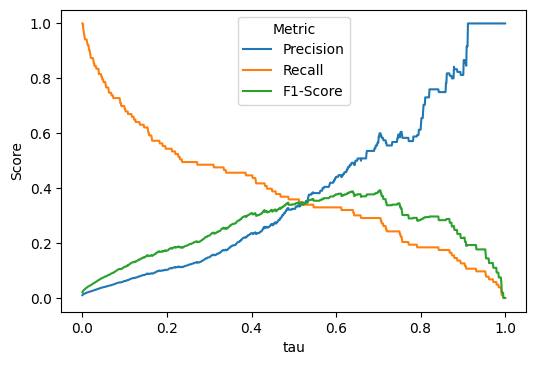
\includegraphics[width=1\linewidth]{gbt_prec_rec_plot.png}
      \caption{GBT}
      \label{fig:gbt_prec_rec_plot}
    \end{subfigure} \\
    \begin{subfigure}{.70\textwidth}
      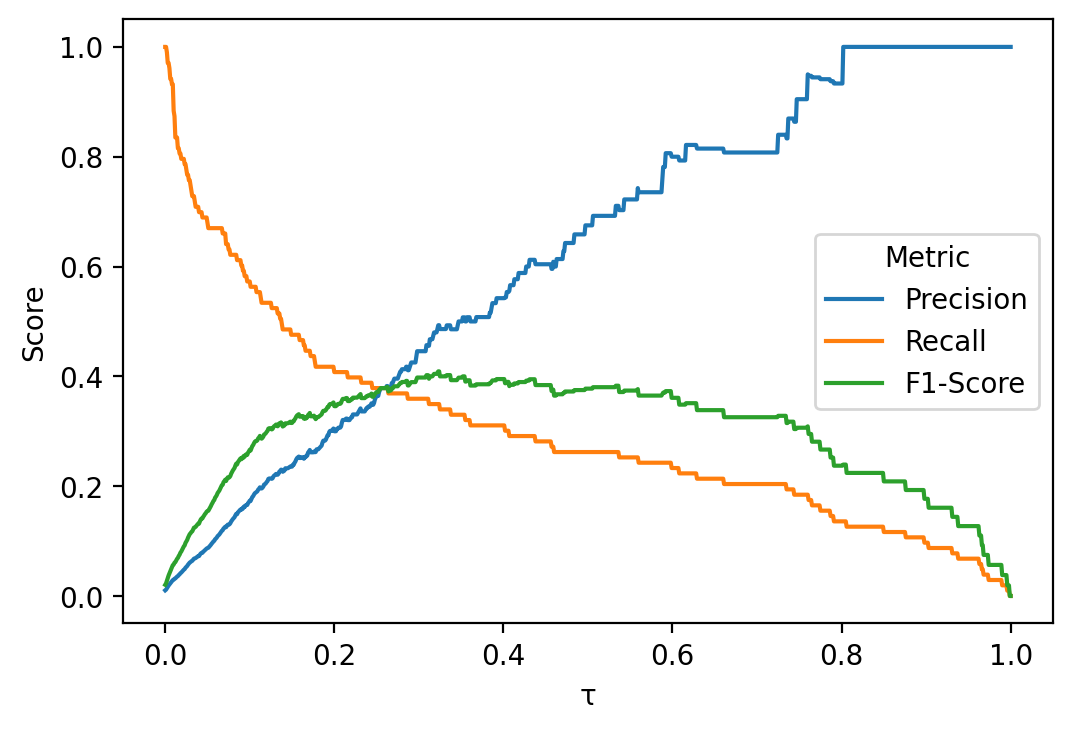
\includegraphics[width=1\linewidth]{ebm_prec_rec_plot.png}
      \caption{EBM}
      \label{fig:ebm_prec_rec_plot}
    \end{subfigure}
    \caption{Comparison of Candidates' Evaluation Metrics for different $\tau$'s}
\label{fig:prec_rec_plot}
\end{figure}
\noindent
The two plots in figure \ref{fig:prec_rec_plot} show, that both candidates for GBT and EBM obtain almost similar evaluation scores, but for different cutoff values $\tau$. Based on the given metrics, a decision in favor of one candidate is therefore not feasible. None of both show dominance in both highly important metrics. We want to emphasize that the comparison of both models should be made on the possible profit increase the models can achieve in the designated setting. This is why the following part will serve as a simplified examplary simulation. \\

\subsubsection*{Examplary Simulation}

As in most applications, the modeller faces a trade-off when selecting the optimal model and/or the optimal $\tau$: High precision versus high recall. How to evaluate this tradeoff typically depends on the costs of false classification on the one hand and the profit of correct classification on the other. \\
We therefore provide a simple simulation for our application on the OOS data set ($N=10,000$), in order to determine the optimal cutoff for both models. First we define a profit-increase-function and its parameters needed. For the function we assume that the models are applied only once to predict potential churners in the subsequent two months. This can be extended to a multi-period setting, but the optimal $\tau$ stays the same. All customers are assumed to have the same net-profit-value (NPV) and all predicted churners ($N^{\hat{C}=1}(\tau)$) receive a rebate $r$ as a churn prevention strategy. Further parameters and their assumption for the simulation are explained in the below table. \\

\begin{table}[h!]
    \centering
    \begin{tabular}{|l|l|l|}
    \hline
    Parameter & Explanation & Value \\
    \hline
    $\Delta \Pi(r, \tau)$ & Profit-Increase to Status-Quo & \\
    $N^{\hat{C}=1}(\tau)$ & Number of predicted Churners & \\
    $p^{prec}(\tau)$ & Precision of Model & \\
    \hline
    $p_{i}^{succ}(r)$ & Probability of Rebate Success & $0.9$ \\
    $NPV_{i}$ & Net-Profit-Value of one Customer & $100$ \\
    $NLV_{i}(r)$ & Net-rebate-Loss-Value of one Customer & $10$ \\
    $K^{RS}$ & Cost per Customer for Rebate Strategy & $2$ \\
    \hline
    \end{tabular}
    \caption{Parameters for Profit-Increase-Simulation}
    \label{tab:paramssim}
\end{table}
\vspace{1mm}
\noindent
The profit-increase to the status-quo due to the model deployment is therefore:
\noindent
\begin{equ}[H]
\begin{equation} \label{profitinc}
    \begin{aligned}
        \Delta \Pi(r, \tau) & = \mathlarger{\sum}_{i=1}^{N^{\hat{C}=1}} p^{prec}p_{i}^{succ}(NPV_{i}-NLV_{i}) - (1-p^{prec})NLV_{i} - K^{RS} \\
        & = N^{\hat{C}=1}(91p^{prec}-12) \\
    \end{aligned}
\end{equation}
\end{equ}
\vspace{1mm}

\noindent
A modeller should search for the $\tau$ which maximizes equation (\ref{profitinc}). It lies in the nature of almost all classification models, that $N^{\hat{C}=1}(\tau)$ negatively depends on $\tau$ and $p^{prec}(\tau)$ has a positive relationship with $\tau$. We again plot the profit increase for 1000 candidates between 0 and 1 for both GBT's and EBM's candidate in figure \ref{fig:prof_increase_plot}.
\begin{figure}[H]
    \centering
    \begin{subfigure}{.7\textwidth}
      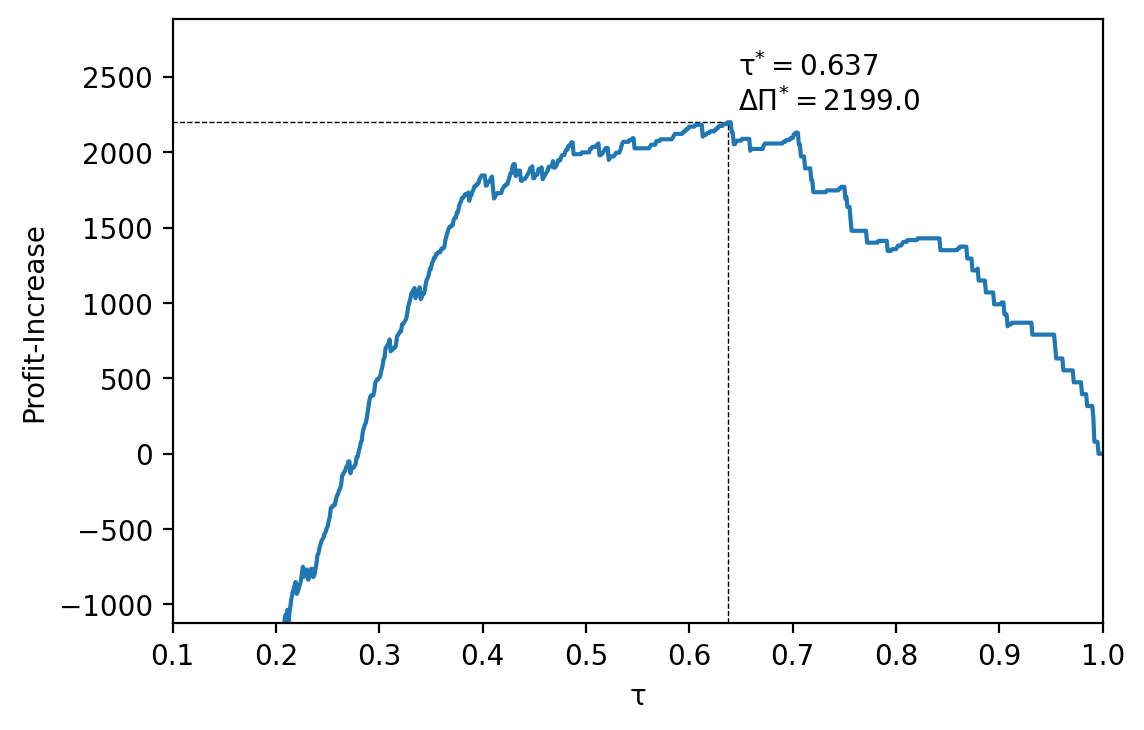
\includegraphics[width=1\linewidth]{gbt_prof_increase_plot.png}
      \caption{GBT}
      \label{fig:gbt_prof_increase_plot}
    \end{subfigure} \\
    \begin{subfigure}{.7\textwidth}
      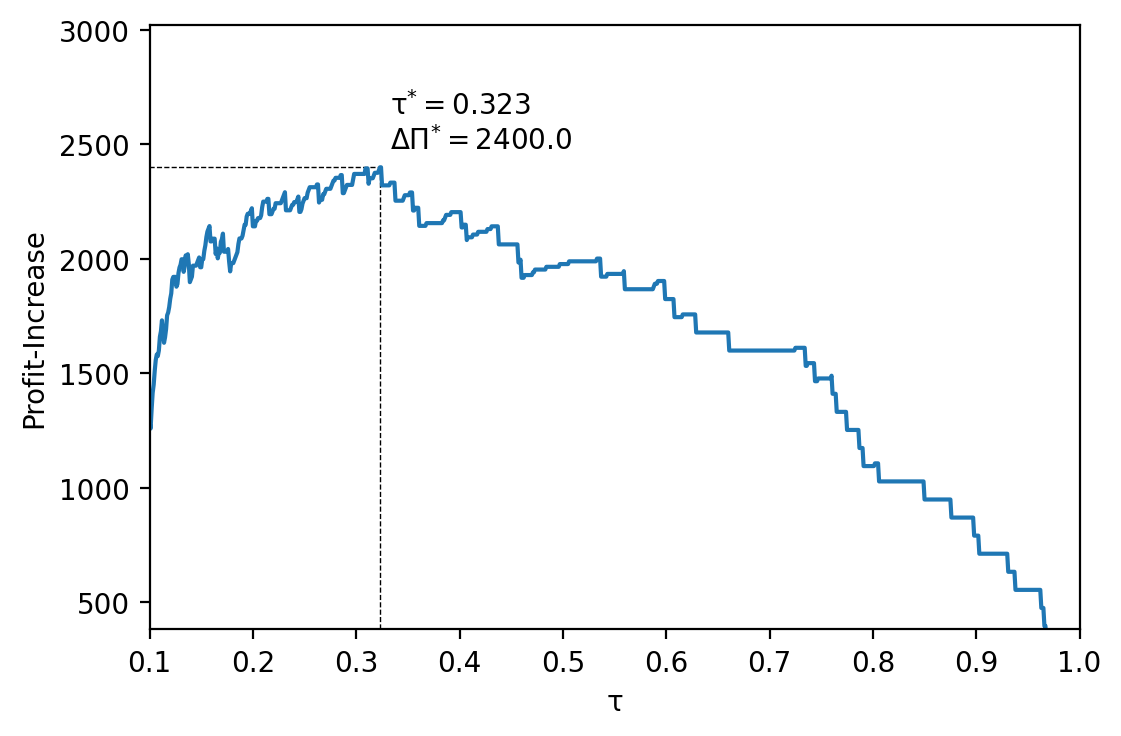
\includegraphics[width=1\linewidth]{ebm_prof_increase_plot.png}
      \caption{EBM}
      \label{fig:ebm_prof_increase_plot}
    \end{subfigure}
    \caption{Profit Increase in Simulation for different $\tau$'s}
\label{fig:prof_increase_plot}
\end{figure}
\noindent
So for our simple simulation the EBM candidate ensures the highest profit increase with a cutoff value $\tau=0.323$. There, with the unseen data at hand, 39\% of churners are detected and the model predicts with a precision of 45\%. Of course, when this simulation approach is applied in practice, the parameters in table \ref{tab:paramssim} should be estimated correctly first. This could result in GBT reaching the profit maximizing cutoff and other optimal precision and recall metrics. The simulation is just an example on how to assess which model has the better KPI-performance and for which cutoff this is ensured. \\

\section{Conclusion} \par

This work presents an applied machine learning approach on a well studied customer churn prediction problem. The emphasize besides high predictive performance is on the predictive power of quotation data on the one hand and interpretability of the modelling approach on the other hand. \\
For the data set and the problem at hand we give insights on all approaches and steps used to get to the reached results. This includes the data preparation, modelling structure, sampling methods, dimension reduction, cost-sensitive loss-functions, machine learning models, evaluation metrics and interpretability approaches. After following the modelling structure we present two candidate models, one for GBT and one for EBM. Both best candidates are achieved with sampling methods and a simple log loss as the objective. \\
In this work we show that quotation data has high predictive power. We therefore want to stress the importance of including in it as explanatory variables. We highly recommend companies and institutions to set up data warehouses which capture quotation activity of customers, which can be used to reflect the current behavior of them. To ensure that the predictive power is generalizable for all companies we want to motivate data collection and further research. The goal is to design a benchmark study on multiple independent data sets examining the benefit of quotation data. \\

Furthermore we want to declare one possible extension of this work which contains a different modelling approach. The idea is to model the events giving the customer the right of mid-contract termination seperately. In the tree diagram of figure \ref{fig:tree_diag} we show how the event sequence leading to a churn is constructed. \\
% Set the overall layout of the tree
\tikzstyle{level 1}=[level distance=5cm, sibling distance=3cm]
\tikzstyle{level 2}=[level distance=5cm, sibling distance=2cm]
% Define styles for bags and leafs
\tikzstyle{bag} = [text width=4em, text centered]
\tikzstyle{end} = [circle, minimum width=3pt,fill, inner sep=0pt]
% The sloped option gives rotated edge labels.
\noindent
\begin{figure}[H]
\begin{tikzpicture}[grow=right, sloped]
\node[bag] {}
    child {
        node[bag] {$None$}
            child {
                node[end, label=right:
                    {$P(None\cap \overline{C})$}] {}
                edge from parent
                node[above] {$P(\overline{C}\mid None)$}
            }
            child {
                node[end, label=right:
                    {$P(None\cap C)$}] {}
                edge from parent
                node[above] {$P(C\mid None)$}
            }
            edge from parent
            node[above] {$P(None)$}
    }
    child {
        node[bag] {$N$}
        child {
                node[end, label=right:
                    {$P(N\cap \overline{C})$}] {}
                edge from parent
                node[above] {$P(\overline{C}\mid N)$}
            }
            child {
                node[end, label=right:
                    {$P(N\cap C)$}] {}
                edge from parent
                node[above] {$P(C\mid N)$}
            }
        edge from parent
            node[above] {$P(N)$}
    }
    child {
        node[bag] {$A$}
        child {
                node[end, label=right:
                    {$P(A\cap \overline{C})$}] {}
                edge from parent
                node[above] {$P(\overline{C}\mid A)$}
            }
            child {
                node[end, label=right:
                    {$P(A\cap C)$}] {}
                edge from parent
                node[above] {$P(C\mid A)$}
            }
        edge from parent
            node[above] {$P(A)$}
    };
\end{tikzpicture}
\caption{Tree Diagram of Events in the mid-contract Churn Setting}
\label{fig:tree_diag}
\end{figure}
\noindent
The tree diagram illustrates how the probability of a churn before the due date can be decomposed using the Events $A$ (Accident), $N$ (New Car) and $C$ (Churn). By assumption we set $P(C\mid None) = 0$ as the amount of terminated contracts during the year which are not being caused by a new car, an accident or a due date is very small and can be omitted. What we are interested in predicting is the overall probability of a churn, which can be rewritten as:
\noindent
\begin{center}
\begin{equation} \label{prob_decomb}
    \begin{aligned}
        P(C) & = P(C\cap A) + P(C\cap A) \\
        & = P(A)P(C\mid A) + P(N)P(C\mid N) \\
    \end{aligned}
\end{equation}
\end{center}
\vspace{1mm}

\noindent
The extension is to seperately model $P(A)$, $P(C\mid A)$, $P(N)$ and $P(C\mid N)$. The best modelling approaches for an accident ($P(A)$) and for a new car ($P(N)$) in $(t, t+s]$ might differ in terms of models, sets of explanatory variables, sampling methods etc. Not only the unconditional but also the conditional probabilities $P(C\cap A)$ and $P(C\cap A)$ may vary in their best modelling approach. Predicting these 4 probabilities seperately can also generate more interpretable insights to the main drivers for a churn. The probability of a churn can be easily recomputed using these 4 quantites and equation (\ref{prob_decomb}). \\

\newpage

\thispagestyle{empty}

\printbibliography

\vspace*{6mm}

\newpage

\thispagestyle{empty}

\section*{Appendix} \par

\subsection*{A. Gradient and Hessian for Weighted Loss Function} \par
\vspace*{6mm}
\noindent
Simple Weighted Loss Function for one sample:
\begin{center}
$l(C, \hat{C}) = -\left(\alpha C\log(\hat{C}) + (1-\alpha)(1 - C)\log(1 - \hat{C})\right)$
\end{center}
\noindent
We perform a few transformations to simplify the derivation:
\begin{center}
    $\alpha_j = \begin{cases} \alpha,& C = 1 \\ 1 - \alpha,& C = 0 \end{cases}$\,\,\,\,\,\, ,\,\,\,\,\,\, $\hat{C}_j = \begin{cases} \hat{C},& C = 1 \\ 1 - \hat{C},& C = 0 \end{cases}$
\end{center}
\noindent
This way the loss simplifies to:
\begin{center}
    $l(C, \hat{C}) = -\alpha_j \log(\hat{C}_j)$
\end{center}
\noindent
Again, consider following rewriting and note these functional relationships:
\begin{itemize}
    \item $\hat{C}_j = \frac{\hat{C}(C+1)}{2} + \frac{(1-\hat{C})(1-C)}{2}$
    \item $\hat{C} = \frac{1}{1+e^{-g(X)}}$
\end{itemize}
\noindent
The Gradient $\frac{\partial l}{\partial g(X)}$ then can be calculated with the chain rule with:
\begin{itemize}
    \item $\frac{\partial l}{\partial \hat{C}_j} = - \frac{\alpha_j}{\hat{C}_j}$
    \item $\frac{\partial \hat{C}_j}{\partial \hat{C}} = \frac{C+1}{2} + \frac{C-1}{2} = C$
    \item $\frac{\partial \hat{C}}{\partial g(X)} = \frac{1}{1+e^{-g(X)}}(\frac{1+e^{-g(X)}}{1+e^{-g(X)}} - \frac{1}{1+e^{-g(X)}}) = \hat{C}(1-\hat{C}) = \hat{C_j}(1-\hat{C_j})$
\end{itemize}
\begin{center}
    \boxed{\frac{\partial l}{\partial g(X)} = \frac{\partial l}{\partial \hat{C}_j}\cdot\frac{\partial \hat{C}_j}{\partial \hat{C}}\cdot\frac{\partial \hat{C}}{\partial g(X)} \,\,\, = \,\,\, - \frac{\alpha_j}{\hat{C}_j}\cdot C\cdot\hat{C}_j(1-\hat{C}_j) \,\,\, = \,\,\, -\alpha_jC(1-\hat{C}_j)}
\end{center}
\vspace*{6mm}
\noindent
The Hessian $\frac{\partial^2 l}{\partial g(X)^2}$ is calculated as:
\begin{center}
    \boxed{\frac{\partial^2 l}{\partial g(X)^2} = \frac{\partial}{\partial \hat{C}_j} \left(\frac{\partial l}{\partial g(X)}\right)\cdot\frac{\partial \hat{C}_j}{\partial \hat{C}}\cdot\frac{\partial \hat{C}}{\partial g(X)} \,\,\, = \,\,\, \alpha_jC^2\hat{C}_j(1-\hat{C}_j)}
\end{center}
\noindent

\newpage

\thispagestyle{empty}

\section*{Appendix} \par

\subsection*{B. Gradient and Hessian for Focal Loss Function} \par
\vspace*{6mm}
\noindent
Focal Loss Function for one sample:
\begin{center}
$l(C, \hat{C}) = -\left(\alpha (1-\hat{C})^{\gamma} C\log(\hat{C}) + (1-\alpha)\hat{C}^{\gamma}(1 - C)\log(1 - \hat{C})\right)$
\end{center}
\noindent
We perform the same transformations to simplify the derivation:
\begin{center}
    $\alpha_j = \begin{cases} \alpha,& C = 1 \\ 1 - \alpha,& C = 0 \end{cases}$\,\,\,\,\,\, ,\,\,\,\,\,\, $\hat{C}_j = \begin{cases} \hat{C},& C = 1 \\ 1 - \hat{C},& C = 0 \end{cases}$
\end{center}
\noindent
This way the loss simplifies to:
\begin{center}
    $l(C, \hat{C}) = -\alpha_j (1-\hat{C})^{\gamma}\log(\hat{C}_j)$
\end{center}
\noindent
Consider following rewriting and note these functional relationships:
\begin{itemize}
    \item $\hat{C}_j = \frac{\hat{C}(C+1)}{2} + \frac{(1-\hat{C})(1-C)}{2}$
    \item $\hat{C} = \frac{1}{1+e^{-g(X)}}$
\end{itemize}
\noindent
The Gradient $\frac{\partial l}{\partial g(X)}$ then can be calculated with the chain rule with:
\begin{itemize}
    \item $\frac{\partial l}{\partial \hat{C}_j} = \alpha_j(1-\hat{C}_j)^{\gamma} \left(\frac{\hat{C}_j\log(\hat{C}_j)^\gamma + \hat{C}_j - 1}{\hat{C}_j(1-\hat{C}_j)}\right)$
    \item $\frac{\partial \hat{C}_j}{\partial \hat{C}} = \frac{C+1}{2} + \frac{C-1}{2} = C$
    \item $\frac{\partial \hat{C}}{\partial g(X)} = \frac{1}{1+e^{-g(X)}}(\frac{1+e^{-g(X)}}{1+e^{-g(X)}} - \frac{1}{1+e^{-g(X)}}) = \hat{C}(1-\hat{C}) = \hat{C_j}(1-\hat{C_j})$
\end{itemize}
\begin{center}
    \boxed{\frac{\partial l}{\partial g(X)} = \frac{\partial l}{\partial \hat{C}_j}\cdot\frac{\partial \hat{C}_j}{\partial \hat{C}}\cdot\frac{\partial \hat{C}}{\partial g(X)} \,\,\, = \,\,\, - \alpha_j(1-\hat{C}_j)^{\gamma} \left(\hat{C}_j\log(\hat{C}_j)^\gamma + \hat{C}_j - 1\right) C}
\end{center}
\vspace*{6mm}
\noindent
The Hessian $\frac{\partial^2 l}{\partial g(X)^2}$ is calculated as:
\begin{center}
    \fbox{%
        \parbox{\textwidth}{
            \centering
            $\mathlarger{\frac{\partial^2 l}{\partial g(X)^2} = \frac{\partial}{\partial \hat{C}_j} \left(\frac{\partial l}{\partial g(X)}\right)\cdot\frac{\partial \hat{C}_j}{\partial \hat{C}}\cdot\frac{\partial \hat{C}}{\partial g(X)} =}$ \\
            \vspace*{2mm}

            $\left(\alpha_j C \gamma (1-\hat{C}_j)^{g-1}\left(\gamma \hat{C}_j \log(\hat{C}_j) + \hat{C}_j - 1 \right)\right)C\hat{C}_j(1-\hat{C}_j) +$ \\
            \vspace*{2mm}

            $\left(\alpha_j C (1-\hat{C}_j)^{\gamma}\left(\gamma\log(\hat{C}_j) + \gamma + 1\right)\right)C\hat{C}_j(1-\hat{C}_j)$
        }%
    }
\end{center}
\noindent


\newpage

\thispagestyle{empty}

\section*{Appendix} \par

\subsection*{C. GBT Perfomance Improvement with Quotation Data} \par

\begin{table}[h!]
    \centering
    \begin{tabular}{|lc|cccccc|}
    \hline
    Model                              & Test-Set & Accuracy        & Precision       & Recall          & F1              & AUROC           & AUPRC            \\ 
    \hline
    \multirow{2}{*}{gbt\_u10\_aNgN}    & OOS      & 0.53\% & 194.56\% & 184.62\%          & 189.86\% & 6.53\%          & 351.17\%           \\ 
    \cdashline{2-8}[1pt/1pt]
                                       & OOP      & 0.60\% & 162.24\% & 84.62\%          & 117.94\%          & 4.05\%          & 236.61\%           \\ 
    \hline
    \multirow{2}{*}{gbt\_d0.1\_aNgN}   & OOS      & 0.08\%          & 85.24\%          & 145.00\%          & 105.23\%          & 3.72\%          & 270.13\%           \\ 
    \cdashline{2-8}[1pt/1pt]
                                       & OOP      & 0.32\%         & 117.86\%          & 131.25\%          & 122.96\% & 1.77\%          & 241.30\%  \\ 
    \hline
    \multirow{2}{*}{gbt\_u\_aNgN}      & OOS      & 4.16\%          & 59.73\%          & 13.79\%          & 54.85\%          & 7.56\%          & 416.18\%           \\ 
    \cdashline{2-8}[1pt/1pt]
                                       & OOP      & 5.39\%         & 69.30\%          & 12.07\%          & 62.63\%          & 5.32\%          & 226.48\%           \\ 
    \hline
    \multirow{2}{*}{gbt\_d0.1\_a0.6gN} & OOS      & -1.97\%          & $\infty$\%         & $\infty$\%          & $\infty$\%          & 80.65\% & 3140.41\%  \\ 
    \cdashline{2-8}[1pt/1pt]
                                       & OOP      & -2.41\%          & $\infty$\%          & $\infty$\%          & $\infty$\%          & 71.53\% & 1544.56\%           \\ 
    \hline
    \multirow{2}{*}{gbt\_u\_a0.8gN}    & OOS      & 55.41\%          & 141.81\%          & -18.28\%          & 131.91\%          & 4.06\%         & 450.51\%           \\ 
    \cdashline{2-8}[1pt/1pt]
                                       & OOP      & 54.86\%          & 99.01\%          & -29.81\%          & 90.49\%          & 1.41\%          & 331.83\%           \\ 
    \hline
    \multirow{2}{*}{gbt\_u50\_aNg0.5}  & OOS      & 0\%          & 0\%          & 0\%          & 0\%          & 0.15\%          & 0.92\%           \\ 
    \cdashline{2-8}[1pt/1pt]
                                       & OOP      & 0\%          & 0\%          & 0\%          & 0\%          & -0.50\%          & -2.34\%           \\ 
    \hline
    \multirow{2}{*}{gbt\_sm\_aNg2}     & OOS      & 3.86\%          & 30.67\%          & 12.33\%         & 29.67\%          & 4.06\%          & 112.34\%           \\ 
    \cdashline{2-8}[1pt/1pt]
                                       & OOP      & 3.34\%          & 8.76\%          & -5.00\%          & 7.95\%          & 2.13\%          & 57.36\%           \\ 
    \hline
    \multirow{2}{*}{gbt\_u50\_a0.6g1}  & OOS      & 20.43\%          & 58.90\%          & -37.67\%          & 50.04\%          & 5.97\%          & 37.30\%           \\ 
    \cdashline{2-8}[1pt/1pt]
                                       & OOP      & 21.37\%          & 39.93\%          & -43.53\%          & 31.95\%          & 6.83\%          & 25.93\%           \\ 
    \hline
    \multirow{2}{*}{gbt\_sm\_a0.7g2}   & OOS      & 0\%          & 0\%          & 0\% & 0\%          & 0\%          & 0\%           \\ 
    \cdashline{2-8}[1pt/1pt]
                                       & OOP      & 0\%          & 0\%          & 0\% & 0\%          & 0\%          & 0\%           \\
    \hline
    \end{tabular}
    \caption{GBT-Candidates Improvement with Quotation Data}
    \label{gbtevalimprov}
\end{table}

\newpage

\thispagestyle{empty}

\section*{Appendix} \par

\subsection*{D. EBM Perfomance Improvement with Quotation Data} \par

\begin{table}[h!]
    \centering
    \begin{tabular}{|lc|cccccc|}
    \hline
    Model                              & Test-Set & Accuracy        & Precision       & Recall          & F1              & AUROC           & AUPRC            \\ 
    \hline
    \multirow{2}{*}{ebm\_none}    & OOS      & 0.15\% & $\infty$\%  & $\infty$\%           & $\infty$\%  & 19.37\%          & 1488.73\%           \\ 
    \cdashline{2-8}[1pt/1pt]
                                       & OOP      & 0.08\% & -23.53\% & 1200.00\%          & 1044.78\%          & 10.13\%          & 373.36\%           \\
    \hline
    \multirow{2}{*}{ebm\_d0.1}   & OOS      & 0.03\%          & 54.59\%         & 109.52\%          & 75.78\%         & 18.54\%          & 176.50\%           \\ 
    \cdashline{2-8}[1pt/1pt]
                                       & OOP      & 0.31\%          & 97.12\%          & 100.00\%          & 98.43\% & 12.29\%          & 174.12\%  \\ 
    \hline
    \multirow{2}{*}{ebm\_d0.5}      & OOS      & 0.14\%          & $\infty$\%          & $\infty$\%          & $\infty$\%          & 26.08\%          & 1691.67\%           \\ 
    \cdashline{2-8}[1pt/1pt]
                                       & OOP      & 0.02\%          & 5.88\%          & 1700.00\%          & 1318.54\%          & 14.26\%          & 475.47\%           \\ 
    \hline
    \multirow{2}{*}{ebm\_d} & OOS      & 5.30\%          & 21.48\%          & 1.22\%          & 20.50\%          & 3.24\% & 20.97\%  \\ 
    \cdashline{2-8}[1pt/1pt]
                                       & OOP      & 6.01\%          & 18.75\%          & -2.20          & 17.65\%          & 1.88\% & 15.41\%           \\ 
    \hline
    \multirow{2}{*}{ebm\_u10}    & OOS      & 0.35\%          & 92.26\%          & 100.00\%          & 95.35\%          & 16.56\%          & 209.98\%           \\ 
    \cdashline{2-8}[1pt/1pt]
                                       & OOP      & 0.64\%          & 124.63\%          & 75.00\%          & 101.49\%          & 9.60\%          & 158.12\%           \\ 
    \hline
    \end{tabular}
    \caption{EBM-Candidates Improvement with Quotation Data}
    \label{ebmevalimprov}
\end{table}

\end{document}